\documentclass[amssymb,twocolumn,aps]{revtex4}
\usepackage[T1]{fontenc}
% allows special characters (including æøå)
\usepackage[utf8]{inputenc}
%\usepackage [norsk]{babel} %if you write norwegian
\usepackage[english]{babel}  %if you write english
%\usepackage[
%backend=biber,
%style=alphabetic,
%sorting=ynt
%]{biblatex}
\usepackage{amsmath,amssymb,bm}
\usepackage{xcolor}    % set colors
\usepackage{listings}
\lstset{language=Python,basicstyle=\ttfamily\scriptsize,columns=fullflexible,
        keywordstyle=\color{blue!60!black},commentstyle=\color{gray},
        frame=single,framerule=0.3pt,xleftmargin=2pt,xrightmargin=2pt}


\usepackage{physics,amssymb}  % mathematical symbols (physics imports amsmath)
%\usepackage{colortbl}
\usepackage{graphicx}         % include graphics such as plots
\usepackage{hyperref}         % automagic cross-referencing 
\usepackage{float}			  % force placement of tables and figures

\newcommand{\vtheta}{\bm{\theta}}
\newcommand{\vy}{\bm{y}}
\newcommand{\vX}{\bm{X}}
\newcommand{\E}{\mathbb{E}}
\newcommand{\lmax}{\lambda_{\max}}
\newcommand{\lmin}{\lambda_{\min}}
% red marker for statements that must be checked against the code before submission
\newcommand{\todo}[1]{\textcolor{red}{\textbf{[TODO: #1]}}}

\setcounter{dbltopnumber}{2}            % up to 2 full-width floats at the top of a page
\renewcommand{\dbltopfraction}{0.9}     % they may take up to 90 % of the page
\renewcommand{\textfraction}{0.05}

\begin{document}
	
\title{Feed-forward Neural Network \\
    \normalsize FYS-STK4155 - Project 2}
\date{\today}               
\author{Giacomo Saporetti, Amanda Rae Josephine, Narne Abhinav Chowdhary}
\affiliation{University of Oslo}

\newpage
	
\begin{abstract}
We implement a feed-forward neural network (FFNN) in NumPy, verify its backpropagation gradients against JAX automatic differentiation and central finite differences, and evaluate it on noisy Runge-function regression and MNIST digit classification. For regression, we compare sigmoid, ReLU and leaky ReLU networks trained using gradient descent, RMSprop and Adam with degree-11 ordinary least squares (OLS), Ridge and Lasso models. Model selection uses five-fold cross-validation (CV) on 80 observations, followed by evaluation on a held-out set of 20 observations. The best networks achieve CV MSE of about $0.016$, close to the observed noise floor of $0.015$, and test MSEs of $0.0127$--$0.0131$, compared with $0.0226$ for OLS. Network architecture has a limited effect on performance, with 66 of the 75 configurations falling within one standard error of the best result, while L1 and L2 regularization provide no clear improvement. On MNIST, the selected $(128,64)$ network achieves $97.56\,\%$ test accuracy, compared with $92.57\,\%$ for Scikit-Learn logistic regression, $92.68\,\%$ for our softmax-only classifier and $97.79\,\%$ for Scikit-Learn's multilayer perceptron. Overall, the results show  that neural networks can outperform traditional regression models, but increasing network complexity or adding regularization does not necessarily lead to better performance.
\end{abstract}

\maketitle

\section{Introduction}
\label{sec:introduction}
Feed-forward neural networks (FFNNs) are widely used in machine learning because they can learn nonlinear representations directly from data, rather than relying on manually selected features. In our previous work \cite{project1}, we approximated the one-dimensional Runge function using polynomial regression with OLS, Ridge, and Lasso, where the input features were explicitly defined as powers of $x$. In contrast, an FFNN learns its own representation through hidden layers. Although the universal approximation theorem \cite{hornik1989} establishes the expressive capabilities of neural networks, it does not guarantee successful optimization or better generalization than classical methods. This motivates a comparison of their performance under different training conditions.

We investigate two problems. The first is regression of the Runge function,$f(x)=1/(1+25x^2)$, using the polynomial models from our previous work as benchmarks \cite{project1}. The second is multiclass classification on the full MNIST dataset \cite{lecun}, where logistic regression, equivalent to a network without hidden layers, serves as a baseline to assess the benefits of hidden layers. We further compare our FFNN with Scikit-Learn's MLPClassifier to evaluate the performance of our implementation against an established reference.

To address these problems, we implement an FFNN from scratch in Python, supporting a flexible number of layers and neurons, selectable hidden activation functions (sigmoid, ReLU, and leaky ReLU), and optional $L_1$ and $L_2$ regularization. The network uses MSE for regression and softmax cross-entropy for classification, with gradients computed through backpropagation and verified against JAX automatic differentiation \cite{jax2018}. We compare gradient descent, RMSprop \cite{tieleman2012}, and Adam \cite{kingma2015}, and examine how network architecture, learning rate, and regularization affect performance. Hyperparameter heatmaps are used to analyse the regression results, while a confusion matrix provides further insight into classification errors. Model selection is performed using validation data, with held-out test sets reserved for final evaluation.

The report is organized as follows. Section~\ref{sec:methods} presents the theoretical framework, followed by the implementation and experimental methodology in Section~\ref{sec:implementation}. Section~\ref{sec:results} presents the regression and classification results, and Section~\ref{sec:discussion} discusses their impliations and limitations, particularly regarding model complexity, optimization, and generalization. Finally, Section~\ref{sec:conclusion} summarizes the main findings and outlines directions for future work. The source code is available in our GitHub repository \footnote{https://github.com/AmandaRaeJ16/FYS-STK4155-Project2}.

\section{Theory and Methods}\label{sec:methods}
\subsection{Cost functions and gradients}
Let $N$ be the number of samples, $y_i$ the targets and $\tilde{y}_i$ the model outputs.
We consider three cost functions, with and without regularization: the mean squared error (MSE) for regression, the binary cross-entropy (BCE) for binary classification, and the softmax cross-entropy (CE) for multiclass classification. Only the MSE and CE are used in the numerical experiments.

\paragraph{Mean squared error.}
\begin{equation}
L_{\mathrm{MSE}} = \frac{1}{N}\sum_{i=1}^{N}\left(y_i-\tilde{y}_i\right)^2,
\qquad
\frac{\partial L_{\mathrm{MSE}}}{\partial \tilde{y}_i} = -\frac{2}{N}\left(y_i-\tilde{y}_i\right).
\end{equation}

\paragraph{Binary cross-entropy.}
With $y_i\in\{0,1\}$ and $\tilde{y}_i\in(0,1)$ the predicted probability of the positive class,
\begin{equation}
L_{\mathrm{BCE}} = -\frac{1}{N}\sum_{i=1}^{N}\left[y_i\log\tilde{y}_i+(1-y_i)\log(1-\tilde{y}_i)\right],
\end{equation}
\begin{equation}
\frac{\partial L_{\mathrm{BCE}}}{\partial \tilde{y}_i}
= \frac{1}{N}\left(-\frac{y_i}{\tilde{y}_i}+\frac{1-y_i}{1-\tilde{y}_i}\right)
= \frac{1}{N}\,\frac{\tilde{y}_i-y_i}{\tilde{y}_i(1-\tilde{y}_i)}.
\end{equation}
If $\tilde{y}_i=\sigma(z_i)$, the gradient with respect to the logit simplifies to $\partial L_{\mathrm{BCE}}/\partial z_i=(\tilde{y}_i-y_i)/N$.

\paragraph{Softmax cross-entropy.}
For $C>2$ classes, the network outputs logits $z_{ic}$ which the softmax maps to probabilities,
\begin{equation}
\tilde{y}_{ic}=\frac{e^{z_{ic}}}{\sum_{k=1}^{C}e^{z_{ik}}},
\end{equation}
and, with one-hot targets $y_{ic}$,
\begin{equation}
L_{\mathrm{CE}} = -\frac{1}{N}\sum_{i=1}^{N}\sum_{c=1}^{C}y_{ic}\log\tilde{y}_{ic}.
\end{equation}
The gradient with respect to the probabilities is $-\frac{1}{N}\,y_{ic}/\tilde{y}_{ic}$, but when combined with the softmax the gradient with respect to the logits reduces to
\begin{equation}
\label{eq:ce_grad}
\frac{\partial L_{\mathrm{CE}}}{\partial z_{ic}}=\frac{1}{N}\left(\tilde{y}_{ic}-y_{ic}\right),
\end{equation}
which is the expression used in backpropagation.

\paragraph{Regularization.}
For any of the losses above, the regularized cost is
\begin{equation}
L_{\mathrm{reg}} = L + \lambda\,\Omega(w),\qquad \lambda\ge 0,
\end{equation}
where $w$ collects all weights (biases are not regularized) and
\begin{equation}
\Omega_{L_1}(w)=\sum_j|w_j|,\qquad \Omega_{L_2}(w)=\sum_j w_j^2 .
\label{eq:penalty}
\end{equation}
The gradient is modified only with respect to the weights:
\begin{align*}
\nabla_w L_{\mathrm{reg}} &= \nabla_w L + \lambda\,\mathrm{sign}(w)\quad(L_1),
\\
\nabla_w L_{\mathrm{reg}} &= \nabla_w L + 2\lambda\, w\quad(L_2),
\end{align*}
where at $w_j=0$ a subgradient is used ($\mathrm{sign}(0)=0$). Setting $\lambda=0$ recovers the unregularized case. 

\subsection{Activation functions}
Each neuron computes $a=f(z)$ with $z=\mathbf{w}^\top\mathbf{x}+b$. The derivative $f'(z)$ enters backpropagation through
\begin{equation}
\frac{\partial C}{\partial z^{(l)}}=\delta^{(l)}=\left(W^{(l+1)\top}\delta^{(l+1)}\right)\odot f'\!\left(z^{(l)}\right).
\end{equation}
We tested three activations in the hidden layers (the softmax above acts only on the output layer).

\subsubsection{Sigmoid.}
\begin{equation}
\sigma(z)=\frac{1}{1+e^{-z}}\in(0,1),\qquad \sigma'(z)=\sigma(z)\bigl(1-\sigma(z)\bigr) .
\end{equation}
The sigmoid is smooth and bounded, but it saturates for large $|z|$, where $\sigma'(z) \to 0$, and it is not zero-centered.

\subsubsection{ReLU.}
\begin{equation}
\mathrm{ReLU}(z)=\max(0,z),\qquad
\mathrm{ReLU}'(z)=\begin{cases}1,&z>0,\\0,&z\le 0,\end{cases}
\end{equation}
where the value of the derivative at $z=0$ is a convention. ReLU does not saturate for $z>0$ and is cheap to compute, but neurons stuck at $z<0$ receive no gradient ("dead" units).

\subsubsection{Leaky ReLU.}
\begin{equation}
\mathrm{LReLU}(z)=\begin{cases}z,&z>0,\\\alpha z,&z\le 0,\end{cases}
\qquad
\mathrm{LReLU}'(z)=\begin{cases}1,&z>0,\\\alpha,&z\le 0,\end{cases}
\end{equation}
with a small slope $\alpha$ (we use $\alpha=0.01$). The gradient never vanishes, which prevents dead units at the cost of one additional hyperparameter.

\subsection{Backpropagation}
For a network with $L$ layers we write $z^{(l)}=W^{(l)}a^{(l-1)}+b^{(l)}$ and $a^{(l)}=f_l\!\left(z^{(l)}\right)$, with $a^{(0)}=x$. The output layer is linear for regression and softmax for classification. For both regression and classification, the chosen output activation and cost function lead to a similar expression for the output error,
\begin{equation}
\delta^{(L)}=\frac{\partial C}{\partial z^{(L)}}\propto\frac{1}{N}\left(\tilde y-y\right),
\end{equation}
with a factor 2 for the MSE as defined above. The error is propagated backwards through the hidden layers with the recursion of the previous subsection, and the gradients with respect to the parameters follow as
\begin{equation}
\frac{\partial C}{\partial W^{(l)}}=\delta^{(l)}\,a^{(l-1)\top}\;(+\text{penalty gradient}),\qquad
\frac{\partial C}{\partial b^{(l)}}=\delta^{(l)} ,
\end{equation}
summed over the samples of a minibatch. One forward and one backward sweep thus yield the gradient with respect to every weight and bias at a cost of roughly two forward passes, independently of the number of parameters. Since $\sigma'(z)\le 1/4$, the error signal is attenuated each time it passes a sigmoid layer, which is the origin of the vanishing gradients measured in Section~\ref{sec:results}.

\section{Implementation and verification} \label{sec:implementation}
\subsection{Code}
The regression network is the class \texttt{ScratchFFNN} (file \texttt{scratch\_ffnn.py}) and the classifier is \texttt{ScratchClassifier} (file \texttt{scratch\_classifier.py}), both written in NumPy\cite{numpy}. Samples are stored in rows, the weight matrix of layer $l$ has shape (inputs, outputs) and the feed-forward step is \texttt{a @ W + b}, so the equations of Section~\ref{sec:methods} appear transposed in the code. The regression network takes the standardized $x$ itself as input. No polynomial design matrix is needed, since the hidden layers learn the features. Architecture, hidden activation, optimizer, learning rate $\gamma$, number of epochs, minibatch size, and penalty type and strength $\lambda$ are arguments of \texttt{fit()}; without hidden layers, the classifier is multinomial logistic regression. Training and validation losses are recorded at every epoch, and a diverging run is flagged and its divergent epoch discarded. Biases are initialized to zero and weights drawn from $\mathcal{N}(0,\sigma^2)$, with $\sigma=\sqrt{2/d_{in}}$ in ReLU and leaky ReLU layers (He initialization \cite{he2015}) and $\sigma=\sqrt{1/d_{in}}$ in sigmoid and output layers, which keeps the variance of the pre-activations approximately constant across layers at initialization.

\subsection{Verification}
The backpropagation of \texttt{ScratchFFNN} is verified with the function \texttt{check\_gradients}. For a network with hidden layers $(8,6,4)$ (one input, 103 parameters) and each of the three hidden activations, every weight and bias agrees with the gradient from \texttt{jax.grad} \cite{jax2018} and with central finite differences, evaluated on the first cross-validation fold of the regression data. The same two checks pass for every parameter of the classifier, both without hidden layers (7850 parameters) and with hidden layers $(8,6)$ for each activation (6404 parameters), on 20 MNIST images. This verifies the softmax--cross-entropy gradient of Eq.~\eqref{eq:ce_grad} independently of the regression code.

\subsection{Optimizers}
Plain gradient descent (GD) uses the full training set, so one epoch is one update $\theta\leftarrow\theta-\gamma g$. For stochastic gradient descent with RMSprop \cite{tieleman2012} and Adam \cite{kingma2015}, we use minibatches of 32 samples (128 for MNIST), so that an epoch has $\lceil n_\text{train}/32\rceil$ updates. RMSprop divides the gradient by the square root of a running average of its square, and Adam additionally keeps a running average of the gradient (momentum) and corrects both averages for their initial bias. Both thus make the step of each parameter of order $\gamma$, irrespective of the gradient magnitude. We use $\beta_1=0.9$, $\beta_2=0.999$, $\epsilon=10^{-8}$ for Adam and a decay rate of $0.9$ for RMSprop, and compare optimizers by the number of parameter \textit{updates} rather than epochs.

\subsection{Regression data and validation of the models}
We draw $n=100$ points $x_i$ uniformly in $[-1,1]$ (seed 2026) with $y_i=f(x_i)+\varepsilon_i$, $\varepsilon_i\sim\mathcal N(0,0.1^2)$ (Fig.~\ref{fig:data}), split 80/20 with the same random state as in our previous work \cite{project1}, so that all models are trained and tested on the same points. Model selection uses 5-fold cross-validation on the 80 training points, with shuffled folds (seed 2026) shared by all models; inputs and targets are standardized with scalers fitted on the training part of each fold, and the validation MSE is reported in the original units.

Because a network is trained for many epochs, the CV error of a setting is defined as the minimum over epochs of the fold-averaged validation curve, and its standard error is the standard error over the five folds at that epoch. This choice includes early stopping in the model selection and makes the CV error slightly optimistic. Settings with a diverging fold are not evaluated after the divergence.  Among the settings with a CV error within one standard error of the best result, we also select the one with the fewest parameters (the one-standard-error rule \cite{hastie2009}).

\begin{figure}[h]
\centering
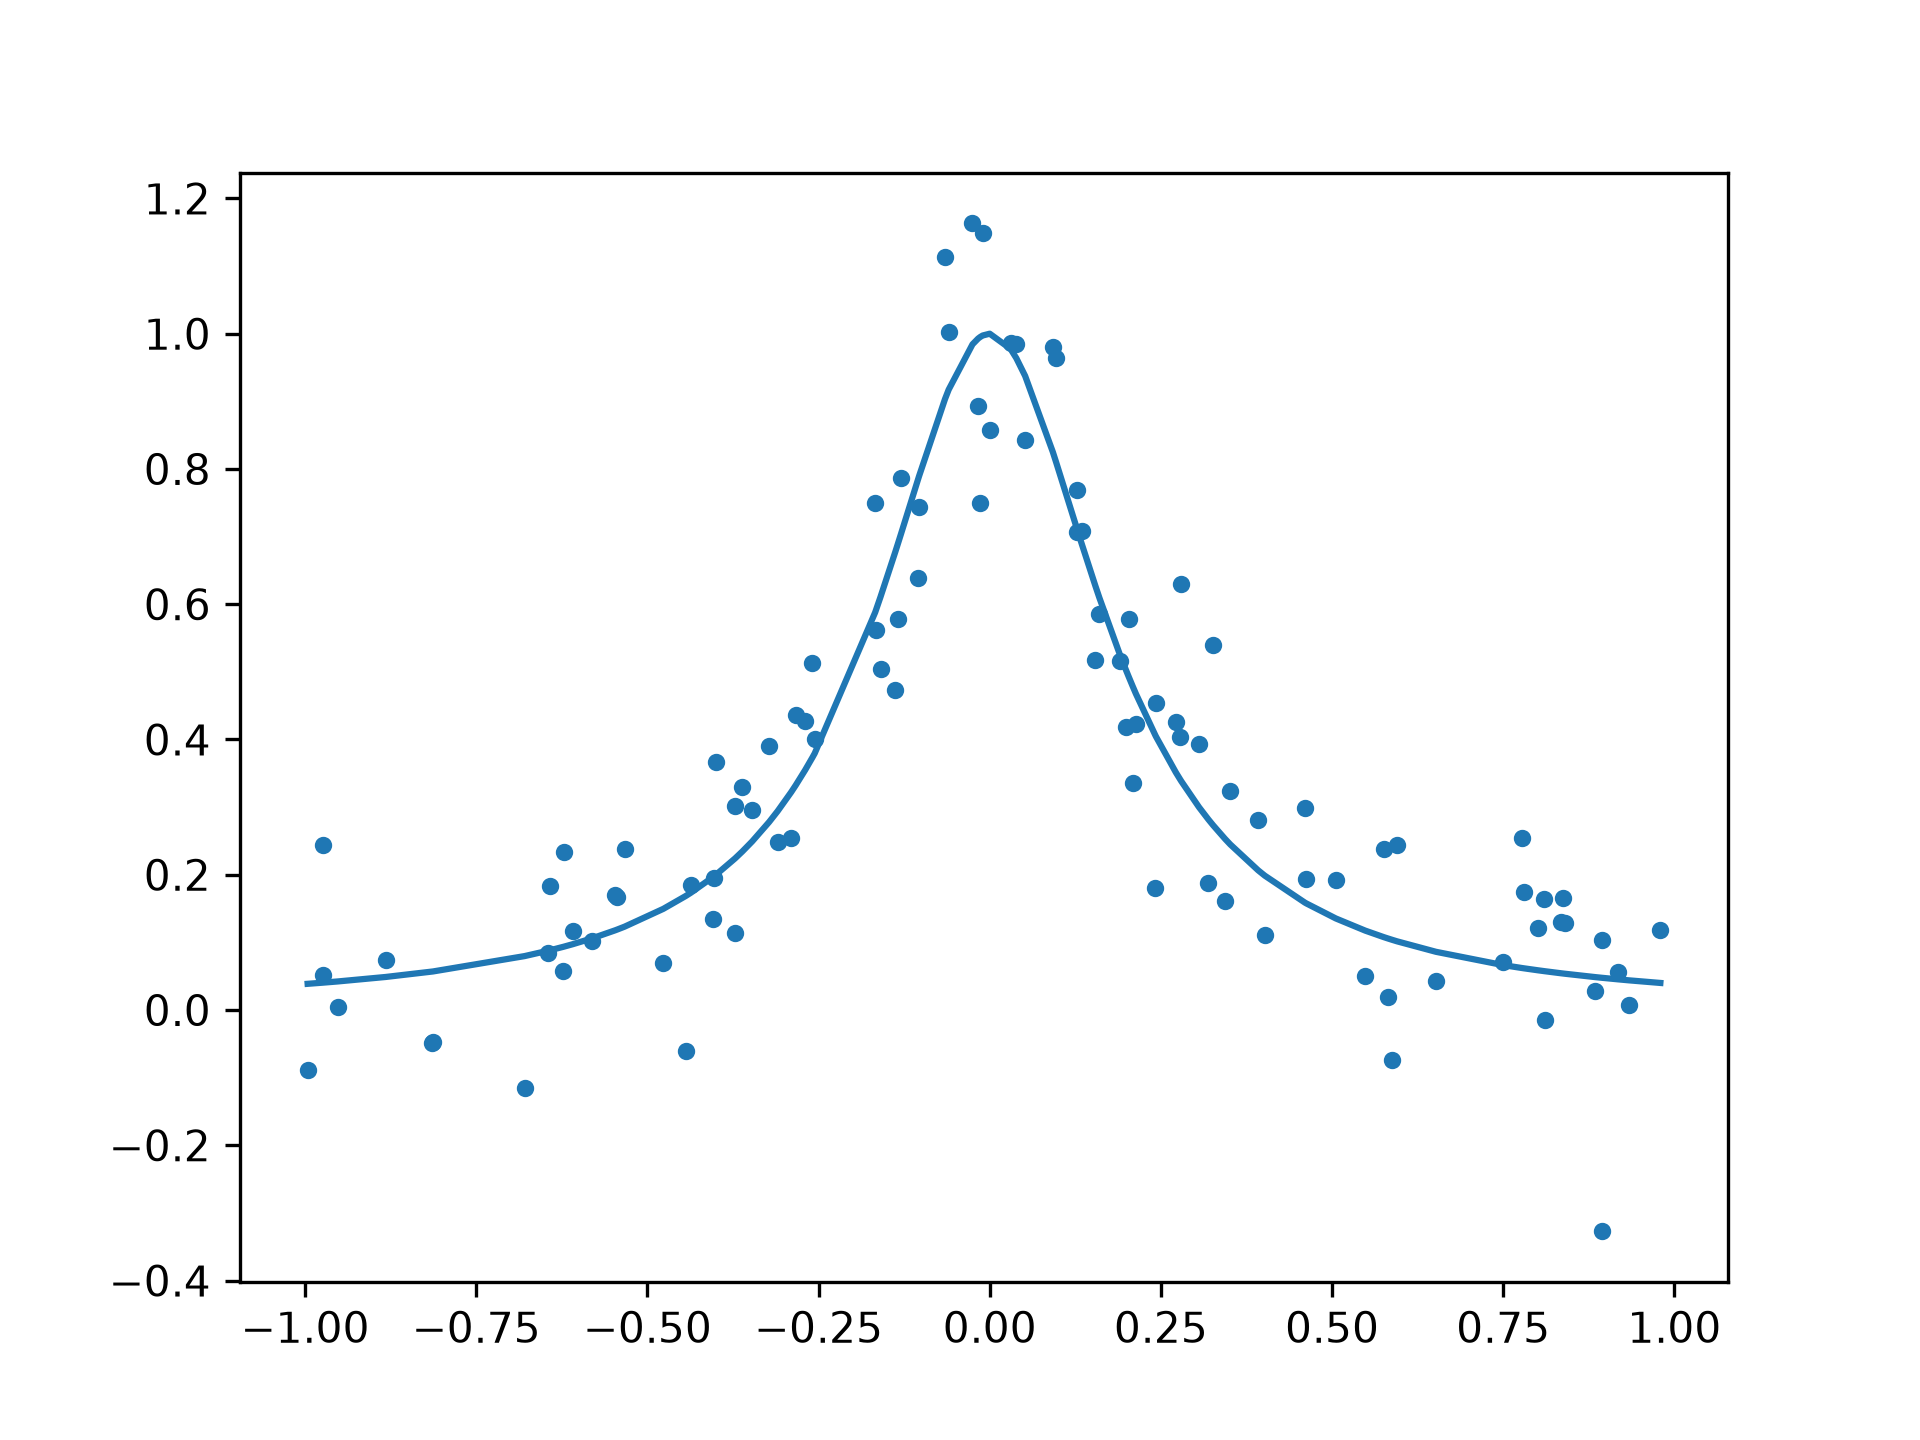
\includegraphics[width=\columnwidth]{figures/fig_data.png}
\caption{The Runge function (line) and the 100 noisy samples ($\sigma=0.1$) used for all regression experiments.}
\label{fig:data}
\end{figure}

The final models are retrained on all 80 points with three weight seeds (42, 43, 44), with the CV-selected number of epochs rescaled to preserve the number of parameter updates (2 per epoch on 64 points, 3 on 80). The true function has an MSE of $0.0150$ on the training points and $0.0096$ on the test points ($\sigma^2=0.01$), which sets the noise floor. We also report the MSE against the noise-free function on 400 grid points, which measures how well the function has been learned independently of the noise in the 20 test points.


\subsection{Polynomial baselines}
The baselines of our previous work \cite{project1} are polynomial models of degree 11 (the best degree found), built with \texttt{PolynomialFeatures}, standardization, and OLS, Ridge or Lasso from Scikit-Learn \cite{pedregosa2011}. The penalty $\lambda$ of Ridge and Lasso is chosen by the same 5-fold CV with the same folds as for the networks, and the test set is used once for the selected $\lambda$. 

\subsection{Classification data and protocol}
MNIST consists of 60\,000 training and 10\,000 test images of $28\times 28$ pixels \cite{lecun}. We flatten the images to 784 features and scale the pixel values to $[0,1]$. A stratified validation set of 6\,000 training images (seed 2026) is set aside, and the networks are trained on the remaining 54\,000 with ReLU, leaky ReLU or sigmoid hidden layers, a ten-node softmax output, the cross-entropy and Adam on minibatches of 128. We scan the learning rate and an $L_2$ penalty for one architecture, then compare five networks at $\gamma=10^{-3}$, $\lambda=10^{-5}$. The test set is used once, for the selected network and the baselines.

The baselines are Scikit-Learn's multinomial logistic regression (\texttt{saga} solver, converged after 511 of at most 1000 iterations, fitted on all 60\,000 images) and our own network without hidden layers, trained like the networks for 20 epochs. As an external reference we train Scikit-Learn's \texttt{MLPClassifier} \cite{pedregosa2011} with the architecture and settings of our selected network (10 epochs, no early stopping) and $\alpha=2\lambda n_\mathrm{batch}=2.56\times10^{-3}$, which reproduces our penalty gradient; only the initialization (Glorot uniform) differs.

\section{Results}\label{sec:results} 
\subsection{Optimizers and learning rates}
\label{sec:optimizers}
We start with the sigmoid networks with one hidden layer of 50 nodes and two layers of 100 nodes, trained with GD (5000 epochs), RMSprop and Adam (1000 epochs) for nine learning rates between $10^{-4}$ and $1$ (Fig.~\ref{fig:blr}, Table~\ref{tab:b}).

\begin{figure*}[t]
\centering
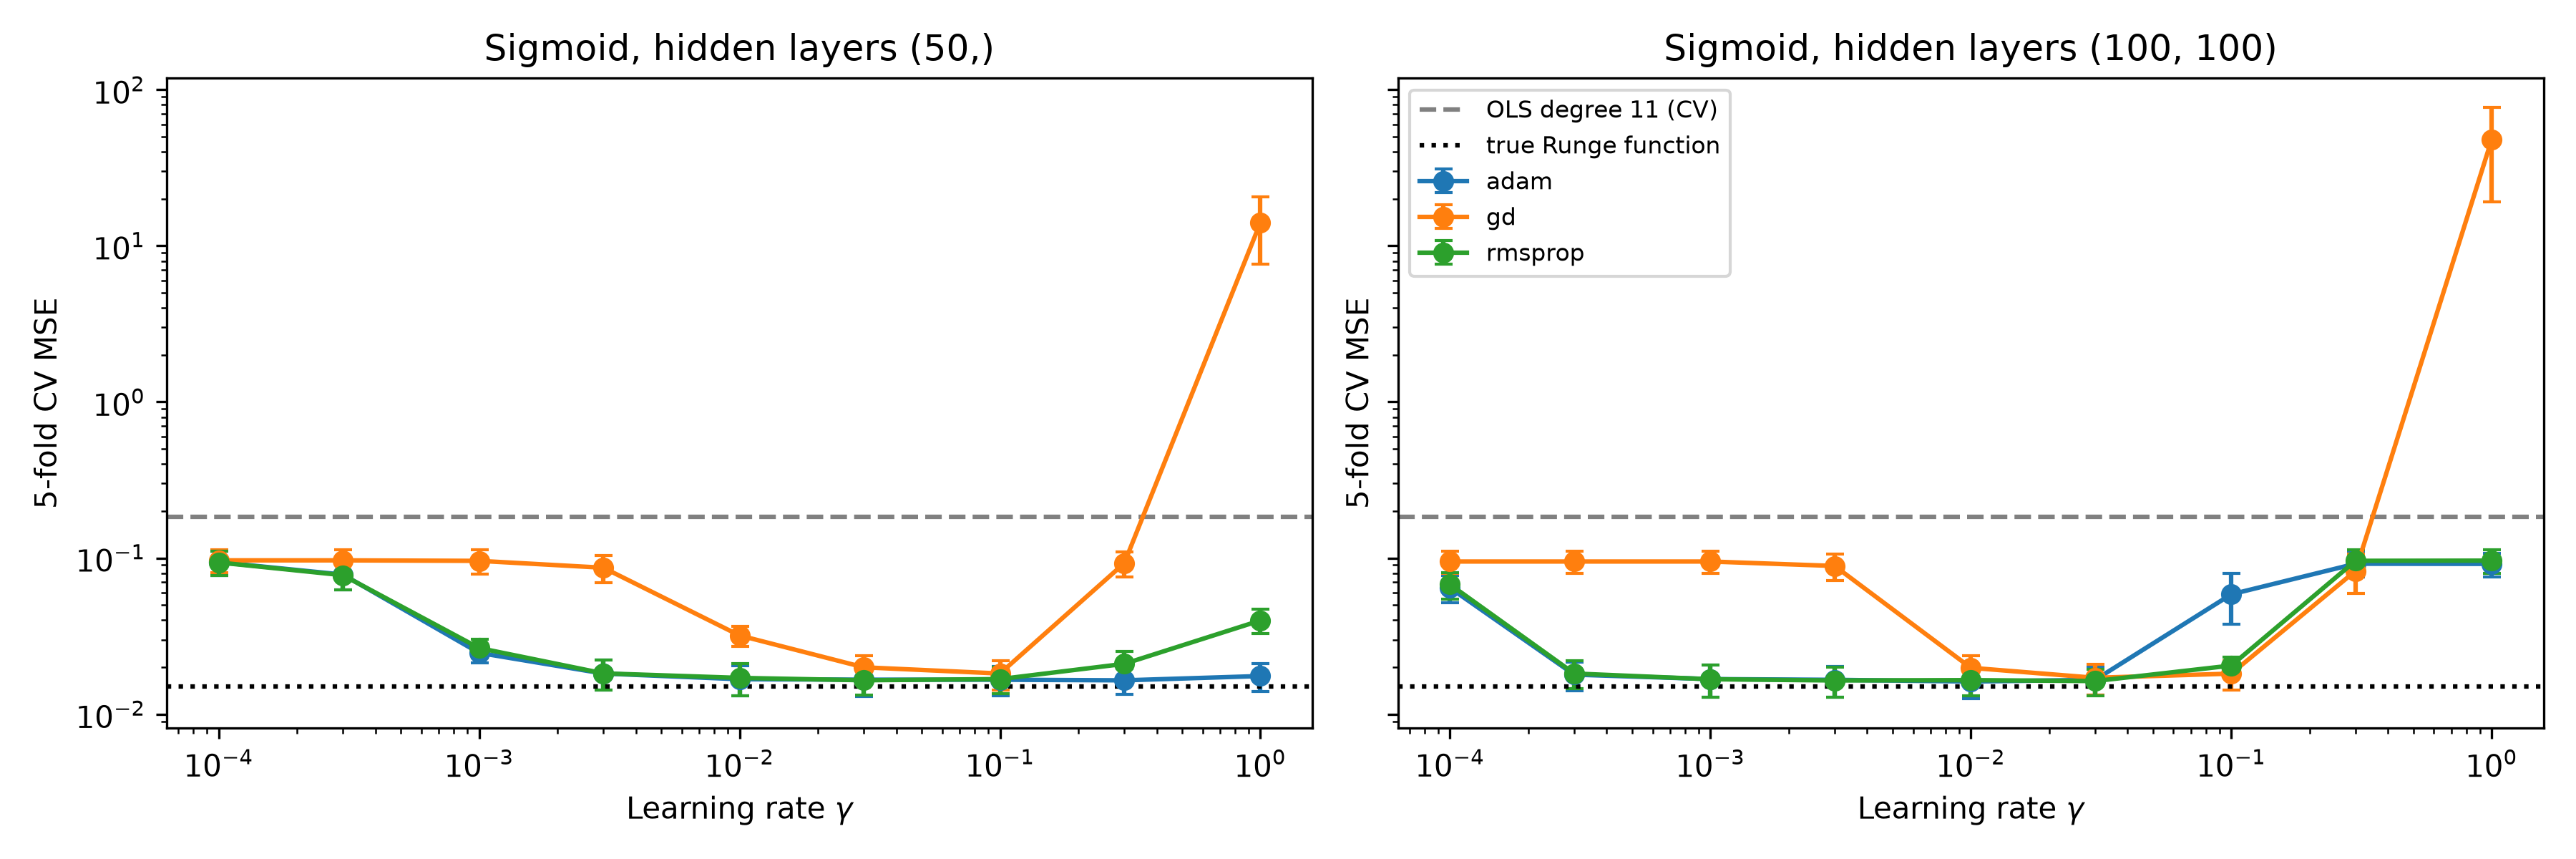
\includegraphics[width=0.85\textwidth]{figures/fig_part_b_lr_scan.png}
\caption{Five-fold CV MSE of the sigmoid networks as a function of the learning rate for GD, RMSprop and Adam. Error bars are the standard error over the folds. The dashed line is OLS of degree 11 and the dotted line the noise floor given by the true Runge function.}
\label{fig:blr}
\end{figure*}

\begin{table}[h]
\centering
\small
\setlength{\tabcolsep}{3pt}
\begin{tabular}{llcccc}
\hline
\textbf{Layers} & \textbf{Opt.} & $\gamma$ & \textbf{CV MSE} & \textbf{SE} & \textbf{Best ep.}\\
\hline
(50,) & GD & 0.1 & 0.0182 & 0.0039 & 5000 \\
(50,) & RMSprop & 0.03 & 0.0165 & 0.0033 & 527 \\
(50,) & Adam & 0.3 & 0.0165 & 0.0031 & 840 \\
(100,100) & GD & 0.03 & 0.0171 & 0.0039 & 5000 \\
(100,100) & RMSprop & 0.03 & 0.0163 & 0.0031 & 167 \\
(100,100) & Adam & 0.01 & 0.0162 & 0.0036 & 319 \\
\hline
\end{tabular}
\caption{Best learning rate of each optimizer for the two sigmoid networks of Part b. For OLS of degree 11 the CV error is $0.183\pm0.142$, and the noise floor is $0.0150$.}
\label{tab:b}
\end{table}

Each optimizer has a window of working learning rates bounded by two failure modes. At small $\gamma$, the CV MSE remains around $0.09$, close to the variance of the targets ($\mathrm{Var}(y)=0.094$), indicating that the networks produce nearly constant predictions and make little progress during training. For GD, this plateau persists up to $\gamma=3\times10^{-3}$ for both architectures. The CV MSE falls below approximately $0.02$ at $\gamma=0.03$–$0.1$ for the $(50,)$ network and $0.01$–$0.1$ for the $(100,100)$ network. At $\gamma=0.3$, the error increases towards the initial plateau, while at $\gamma=1$ it rises sharply to $14$ and $48$, respectively, with two folds diverging for the smaller network.

In contrast, RMSprop and Adam maintain low CV errors across a wider range of learning rates. For the $(50,)$ network, RMSprop achieves a CV MSE below $0.0182$ for $\gamma=3\times10^{-3}$–$0.1$, while Adam remains effective up to $\gamma=1$. For the $(100,100)$ network, both optimizers perform well over $\gamma=3\times10^{-4}$–$0.03$. Their ability to train at smaller learning rates may be attributed to adaptive scaling of parameter updates, which allows them to make progress even when gradients are small. However, their performance remains sensitive to network architecture. While the $(50,)$ network trains successfully with Adam at $\gamma=1$, the $(100,100)$ network deteriorates at $\gamma=0.1$, with CV MSEs of $0.059$ for Adam and $0.020$ for RMSprop, and returns to the high-error plateau for $\gamma\geq0.3$. This suggests that wider networks may respond differently to the same learning rate, although this explanation was not independently tested.



The learning curves in Fig.~\ref{fig:bcurves} further illustrate the differences in convergence speed. For the $(100,100)$ network, GD remains near the initial plateau for approximately $10^3$ parameter updates, compared with $10^2$ for Adam. Moreover, GD achieves its lowest validation error at the final epoch (5000) for both architectures, suggesting that further training may improve its performance. In contrast, RMSprop and Adam reach their minimum validation errors after 167–840 epochs (334–1680 updates), achieving comparable performance with substantially fewer updates.

\begin{figure*}[t]
\centering
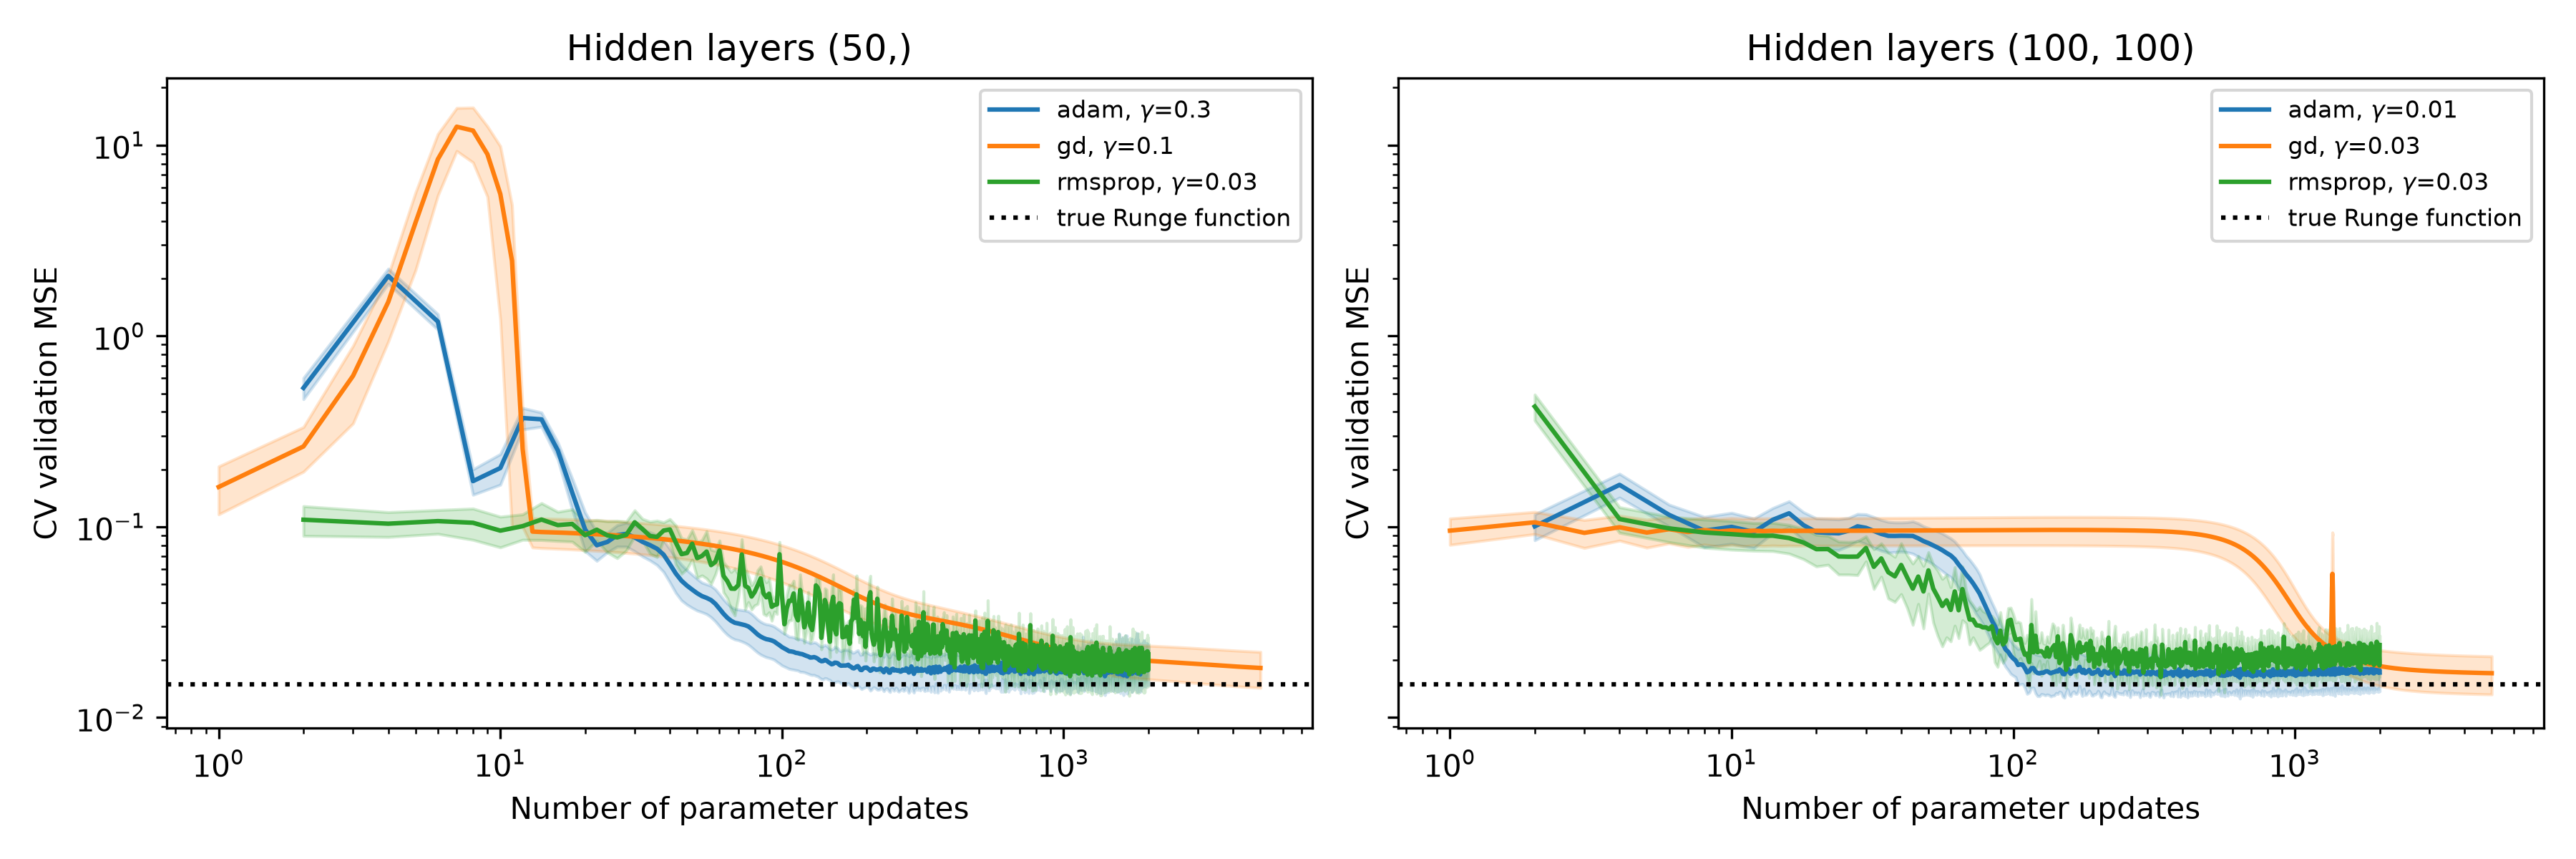
\includegraphics[width=0.85\textwidth]{figures/fig_part_b_curves.png}
\caption{Fold-averaged validation MSE as a function of the number of parameter updates, at the best learning rate of each optimizer (bands: $\pm1$ standard error over folds). Left: $(50,)$. Right: $(100,100)$.}
\label{fig:bcurves}
\end{figure*}

Across the best settings, the CV MSE ranges from $0.0162$ to $0.0182$, approximately 8--21\% above the observed noise floor of $0.0150$. These results are substantially lower than the OLS CV MSE of $0.183\pm0.142$, which is dominated by one poorly performing fold (MSE $0.751$), potentially due to instability near the interval boundaries. However, the differences between the neural network configurations are small (at most $0.002$) relative to their standard errors of $0.003$–$0.004$. Thus, although the adaptive optimizers converge more efficiently than GD, the results provide no clear evidence that either optimizer or network architecture consistently achieves a lower prediction error.

\subsection{Activation functions, depth and width}
\label{sec:architecture}

We first tune the learning rate $\gamma$ for each activation function using Adam on the $(50,50)$ network, as shown in Figure ~\ref{fig:clr}. The lowest CV MSEs are similar across all three activations: $0.0163$ for sigmoid at $\gamma=0.01$, $0.0166$ for ReLU at $\gamma=0.01$, and $0.0164$ for leaky ReLU at $\gamma=0.03$. At smaller learning rates, performance deteriorates, particularly for sigmoid, which reaches a CV MSE of $0.039$ at $\gamma=3\times10^{-4}$. The best learning rate for each activation is subsequently used to compare network architectures.


\begin{figure}[h]
\centering
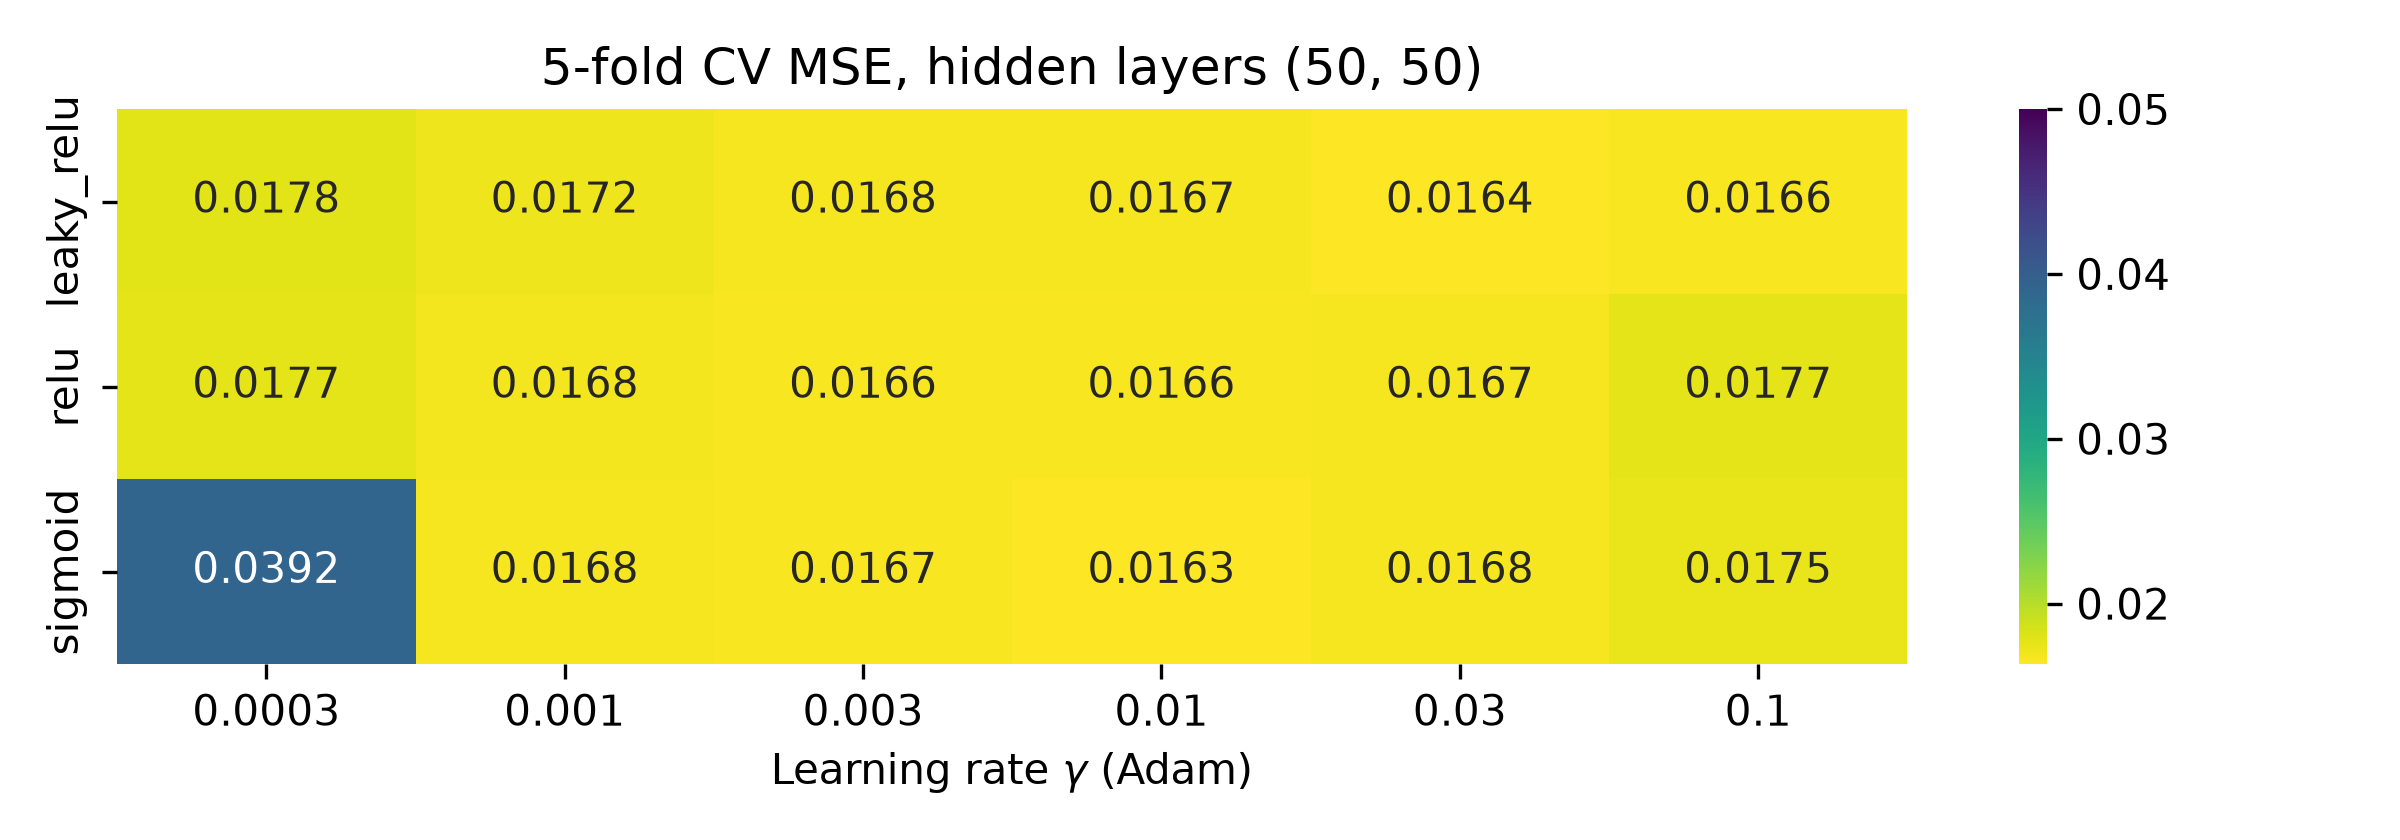
\includegraphics[width=\columnwidth]{figures/fig_part_c_lr_heatmap.png}
\caption{CV MSE of the $(50,50)$ network with Adam for each activation and learning rate.}
\label{fig:clr}
\end{figure}

\begin{figure*}[t]
\centering
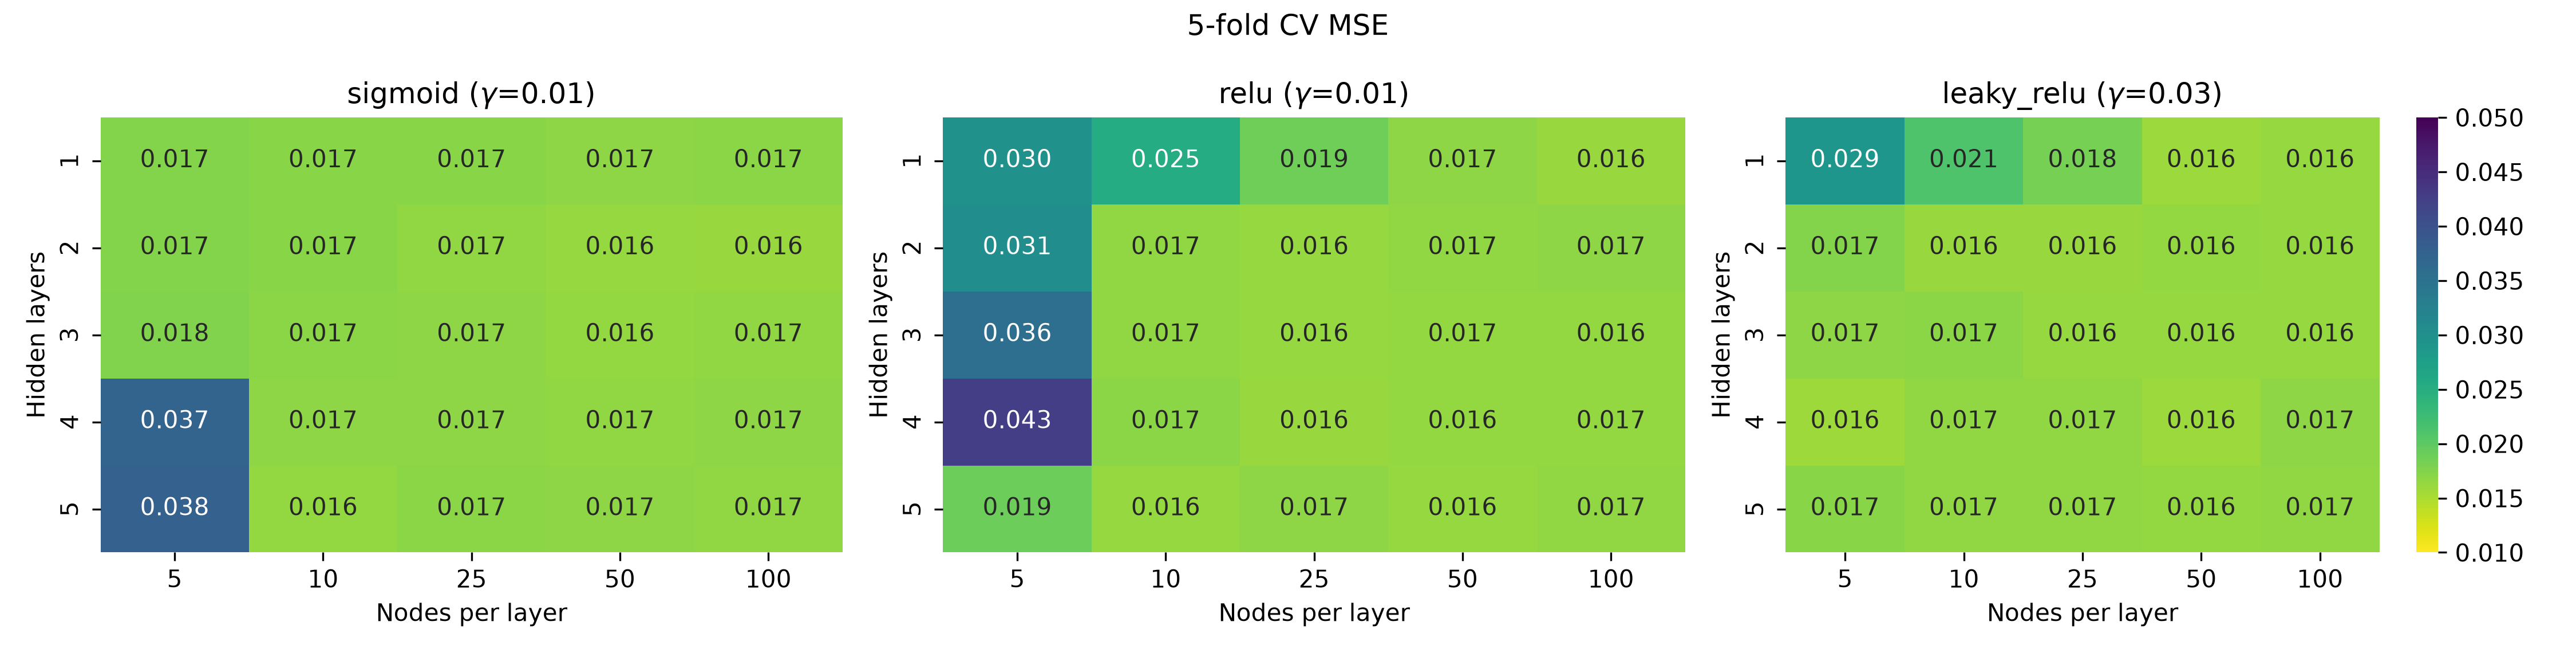
\includegraphics[width=\textwidth]{figures/fig_part_c_depth_width.png}
\caption{Five-fold CV MSE for 1--5 hidden layers and 5--100 nodes per layer, for each activation at its tuned learning rate (Adam, 800 epochs).}
\label{fig:depthwidth}
\end{figure*}

Figure ~\ref{fig:depthwidth}) presents the CV MSE across 75 configurations, covering 1–5 hidden layers with 5–100 nodes per layer. Overall, performance varies little across architectures, with 66 configurations falling within one standard error of the best result. The lowest CV MSE of $0.0159\pm0.0032$ is achieved by a leaky ReLU network with four hidden layers of five nodes each (106 parameters). However, applying the one-standard-error rule selects a much simpler sigmoid network with one hidden layer of five nodes (16 parameters), which achieves a comparable CV MSE of $0.0174\pm0.0037$. This suggests that increasing network complexity does not necessarily improve predictive performance for this regression task.

Despite the generally similar performance, nine configurations have a CV MSE above $0.02$, all involving narrow networks. ReLU networks with five nodes per layer perform poorly at depths of one to four layers (CV MSE $0.030$–$0.043$), as does the single-layer network with ten nodes ($0.025$). The large standard errors for the three- and four-layer configurations ($\approx0.016$) indicate substantial variation across folds. In contrast, leaky ReLU performs poorly only for single-layer networks with five ($0.029$) or ten ($0.021$) nodes, while deeper five-node networks achieve CV MSEs of approximately $0.016$–$0.017$. Since leaky ReLU retains a nonzero gradient for negative pre-activations, these findings are consistent with inactive neurons limiting the performance of narrow ReLU networks, although this mechanism was not directly measured.


Sigmoid networks also show reduced performance in deep, narrow architectures, with CV MSEs increasing to $0.037$ and $0.038$ for four and five hidden layers of five nodes, respectively. In contrast, networks with up to three hidden layers generally maintain CV MSEs of $0.016$–$0.018$. The deterioration in deeper, narrower networks is consistent with the vanishing-gradient problem illustrated in Figure ~\ref{fig:vanishing}. At initialization, a network with ten hidden layers of 50 nodes exhibits a decrease in gradient norm from approximately $2$ near the output to $10^{-7}$ in the first hidden layer. For ReLU and leaky ReLU, the gradient norms remain around $5$ across most layers. The strong attenuation in sigmoid networks is consistent with the bound $\sigma'(z)\leq1/4$, although gradient propagation also depends on the weight matrices.

\begin{figure}[h]
\centering
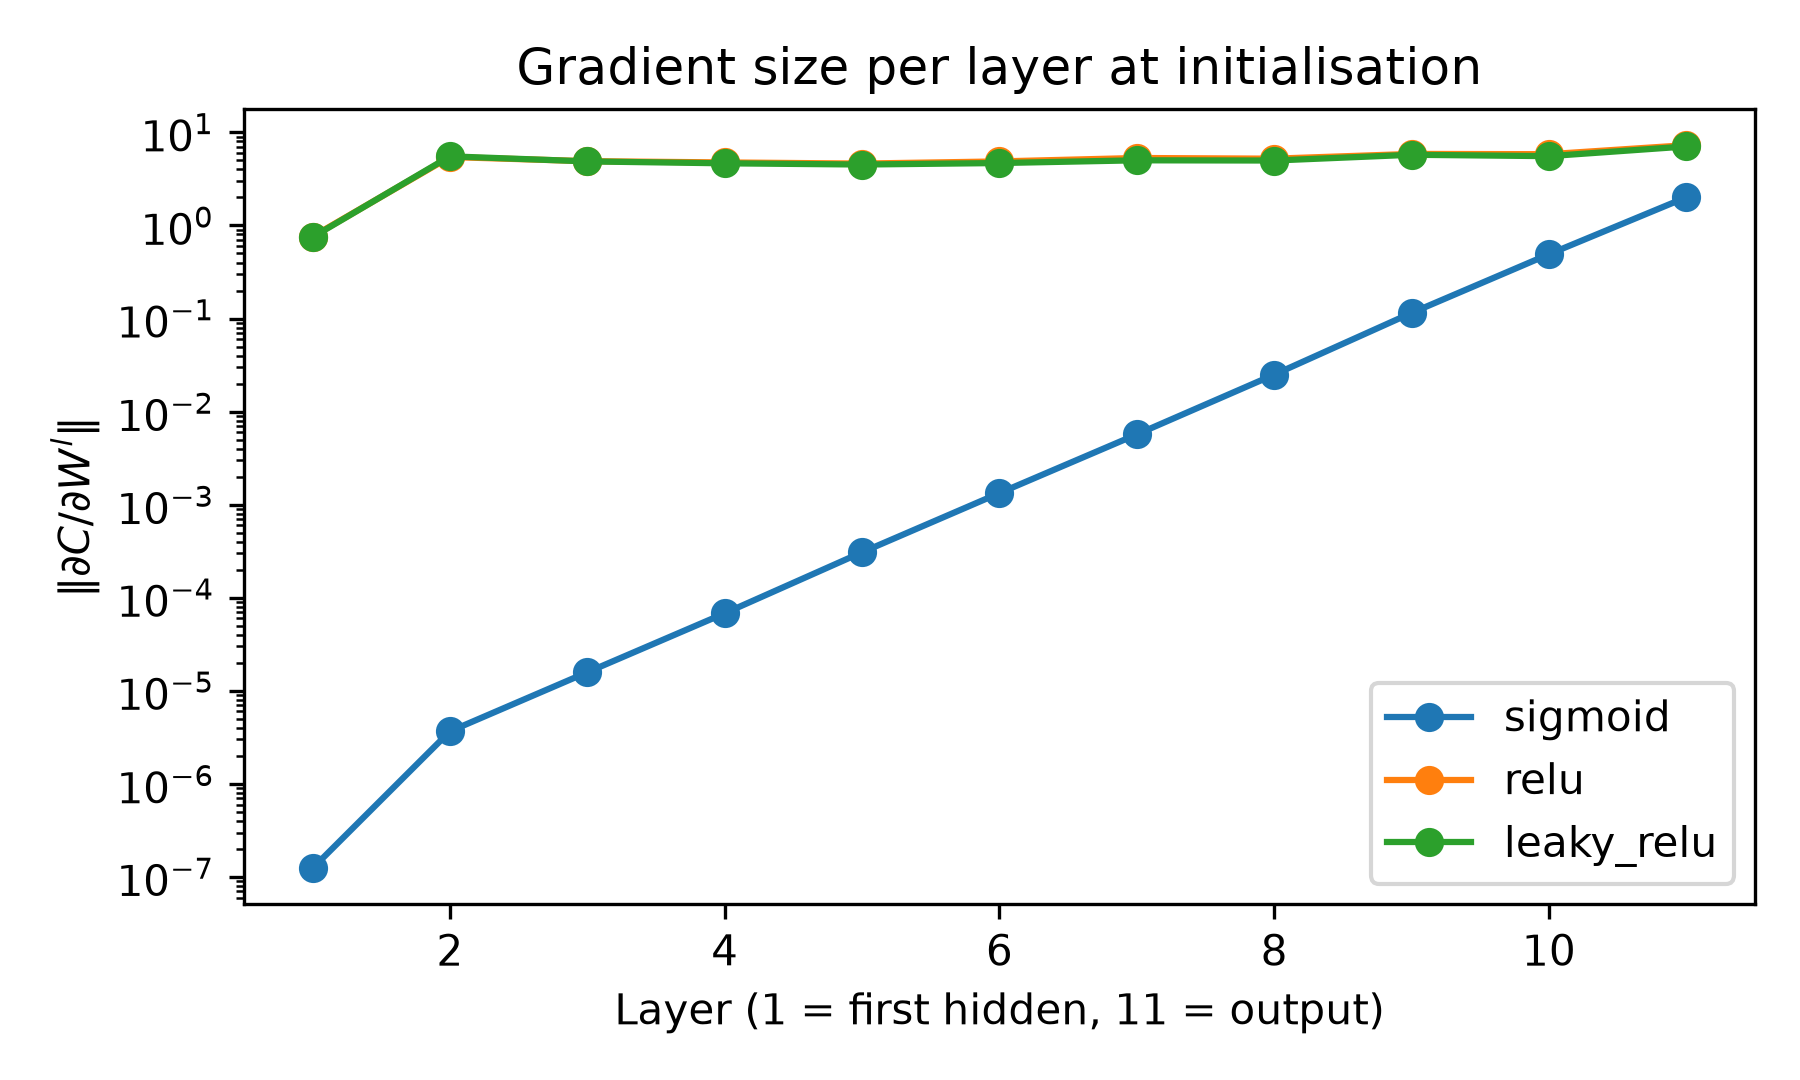
\includegraphics[width=\columnwidth]{figures/fig_part_c_vanishing.png}
\caption{Norm of the gradient with respect to the weights of each layer at initialization, for ten hidden layers of 50 nodes (average of five seeds).}
\label{fig:vanishing}
\end{figure}

Despite this gradient attenuation, wider sigmoid networks with five hidden layers maintain low CV errors. Adam's adaptive parameter updates may help these networks train despite small gradients, although this was not independently tested using GD. Overall, the results suggest that increasing depth or width provides limited improvement once a network is sufficiently expressive, while narrow architectures are more sensitive to the choice of activation function.

\subsection{Overfitting and early stopping}
Figure ~\ref{fig:overfit} illustrates how larger networks can overfit the training data, achieving lower training errors while their validation errors increase. After 800 epochs, three-layer ReLU and leaky ReLU networks with at least 1376 parameters achieve training MSEs of $0.0104$–$0.0115$, below the observed training noise floor of $0.0150$, while their validation MSEs remain higher at $0.021$–$0.026$. In contrast, the sigmoid networks maintain training and validation MSEs of approximately $0.013$ and $0.017$–$0.018$, respectively, showing less evidence of overfitting over the same training period.

To examine this behaviour further, we train the $(100,100,100)$ network for 3000 epochs, as shown in Figure ~\ref{fig:overfit}. The lowest validation MSEs range from $0.0164$ to $0.0166$, reached at epochs 114, 292, and 42 for sigmoid, ReLU, and leaky ReLU, respectively. However, continued training reduces the training MSE to $0.008$–$0.011$ while increasing the validation MSE to $0.021$–$0.030$. Selecting the number of epochs based on the lowest validation error therefore reduces the validation MSE by a factor of approximately $1.3$–$1.6$ compared with using the final epoch. This demonstrates the importance of early stopping in limiting overfitting, particularly for larger networks.

The learning curves also exhibit occasional fluctuations, most noticeably for leaky ReLU after approximately 2000 epochs. With Adam and a constant learning rate, such fluctuations can affect the final validation error and make the results sensitive to numerical differences across runs. In our experiments, the final errors varied by up to $20\%$ across machines, whereas the minimum validation errors remained relatively stable. We therefore base our comparisons on the best validation errors rather than the final-epoch values.

\begin{figure*}[t]
\centering
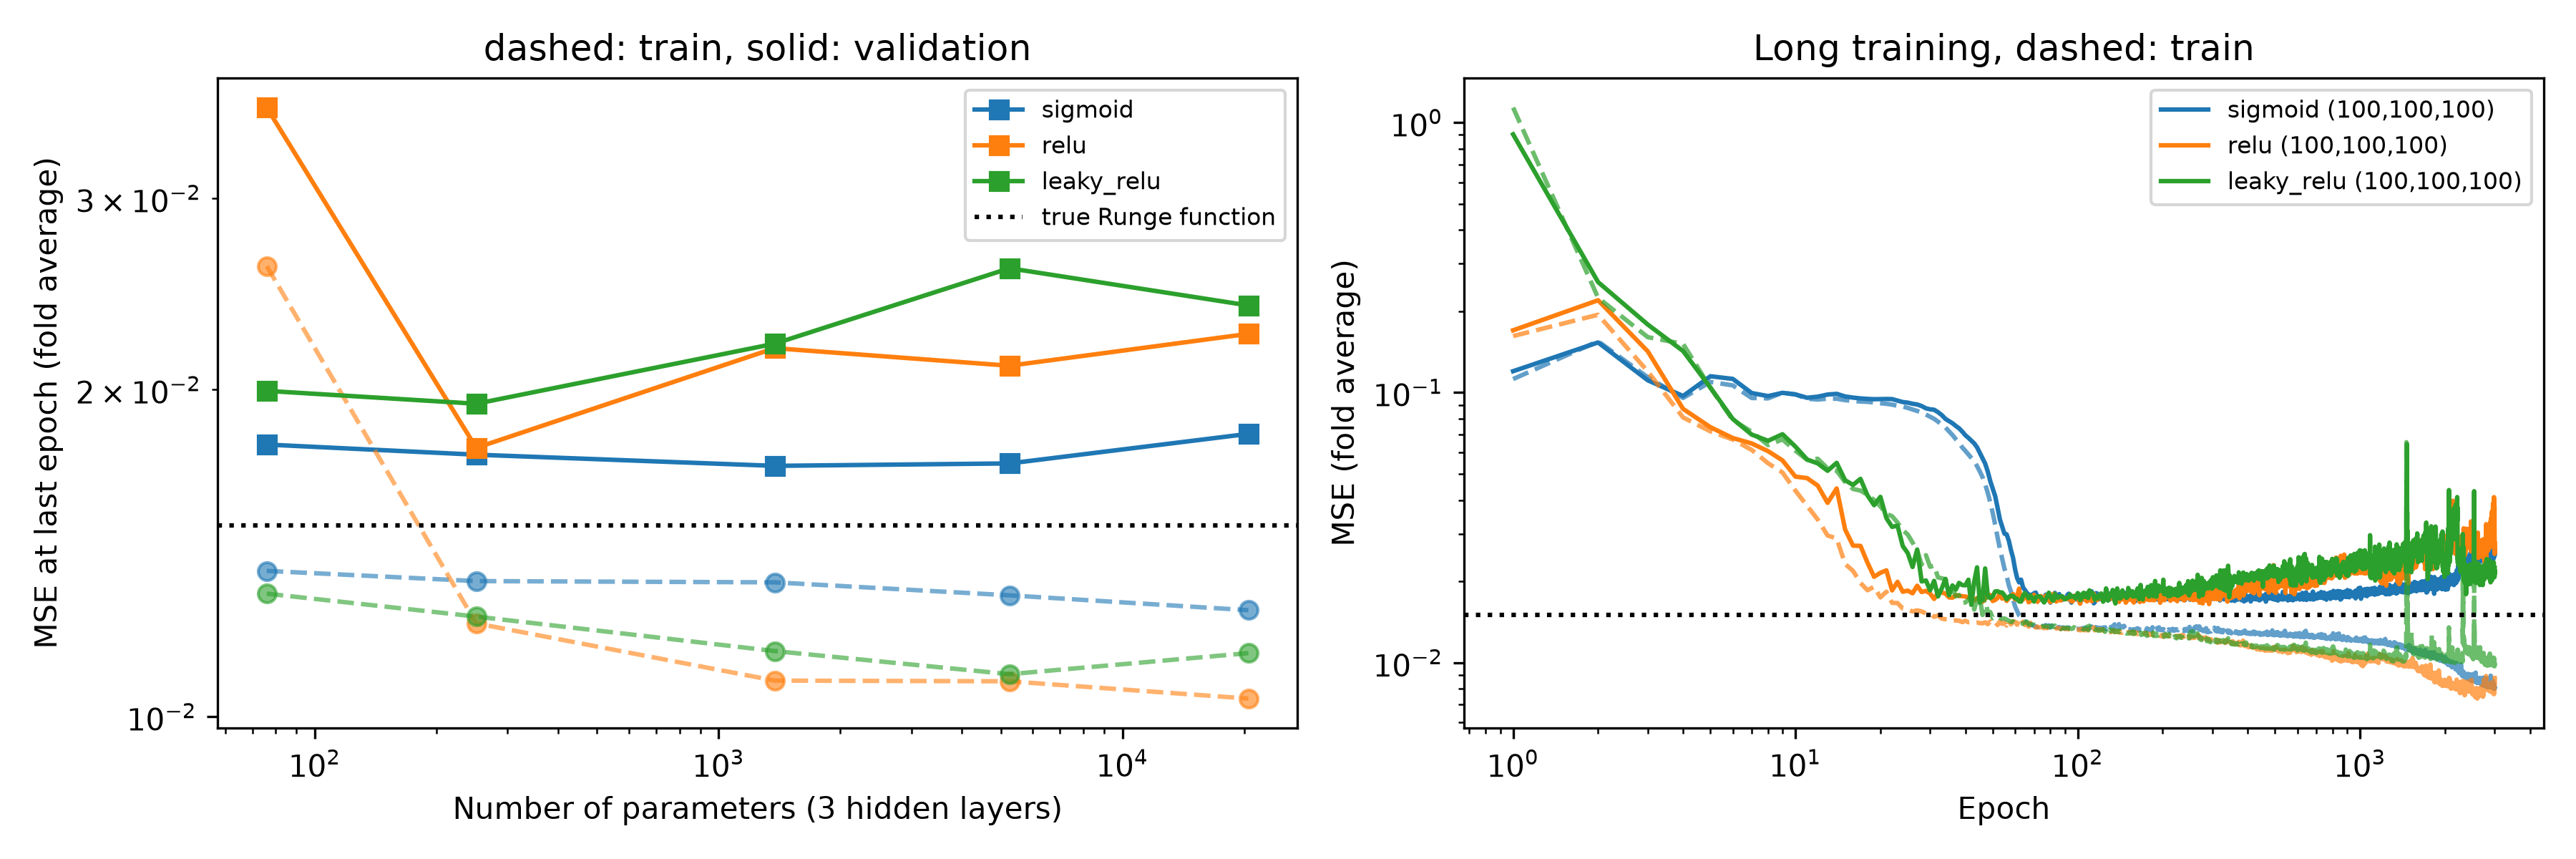
\includegraphics[width=0.85\textwidth]{figures/fig_part_c_overfit.png}
\caption{Left: fold-averaged train (dashed) and validation (solid) MSE at the last epoch against the number of parameters for three hidden layers. Right: long training run of a network with three hidden layers of 100 nodes. The dotted line is the MSE of the true function on the training points.}
\label{fig:overfit}
\end{figure*}

\subsection{Comparison with the polynomial models on the test set}
\label{sec:comparison}
Table~\ref{tab:final} and Fig.~\ref{fig:fits} compare the selected neural networks with the degree-11 regression models on the test set. The networks include the best sigmoid configurations from Section~\ref{sec:optimizers} and the lowest-CV and one-standard-error choices from Section~\ref{sec:architecture}.

\begin{table*}[t]
\centering
\small
\setlength{\tabcolsep}{4pt}
\begin{tabular}{lrcccc}
\hline
\textbf{Method} & \textbf{Params} & \textbf{CV MSE $\pm$ SE} & \textbf{Test MSE} & \textbf{MSE vs.\ true $f$} \\
\hline
True Runge function (noise floor) & -- & $0.0150$ & $0.0096$ & $0$ \\
OLS, degree 11 & 12 & $0.183\pm0.142$ & $0.0226$ & $0.0088$ \\
Ridge, degree 11, $\alpha=0.01$ & 12 & $0.0329\pm0.0077$ & $0.0211$ & -- \\
Lasso, degree 11, $\alpha=10^{-4}$ & 10 & $0.0273\pm0.0065$ & $0.0200$ & -- \\
NN sigmoid $(50,)$, Adam, $\gamma=0.3$ & 151 & $0.0165\pm0.0031$ & $0.0129\pm0.0033$ & $0.0027$ \\
NN sigmoid $(100,100)$, Adam, $\gamma=0.01$ & 10\,401 & $0.0162\pm0.0036$ & $0.0127\pm0.0008$ & $0.0009$ \\
NN leaky ReLU $(5,5,5,5)$, Adam, $\gamma=0.03$ (lowest CV) & 106 & $0.0159\pm0.0032$ & $0.0496\pm0.0570$ & $0.0269$ \\
NN sigmoid $(5,)$, Adam, $\gamma=0.01$ (one-SE rule) & 16 & $0.0174\pm0.0037$ & $0.0131\pm0.0002$ & $0.0010$ \\
NN leaky ReLU $(50,50)$, no penalty$^{*}$ & 2701 & $0.0160\pm0.0035$ & $0.0161$ & -- \\
NN leaky ReLU $(50,50)$, $L_1$ $\lambda=10^{-3}$$^{*}$ & 2701 & $0.0156\pm0.0029$ & $0.0173$ & -- \\
NN ReLU $(50,50)$, $L_2$ $\lambda=10^{-2}$$^{*}$ & 2701 & $0.0156\pm0.0040$ & $0.0305$ & -- \\
\hline
\end{tabular}
\caption{Regression results. The test MSE of the networks of Parts b and c is the mean $\pm$ standard deviation over three seeds. $^{*}$: networks of Part d, trained with one seed only (see Section~\ref{sec:partd}). The last column is the MSE with respect to the noise-free function on 400 grid points.}
\label{tab:final}
\end{table*}

\begin{figure}[h]
\centering
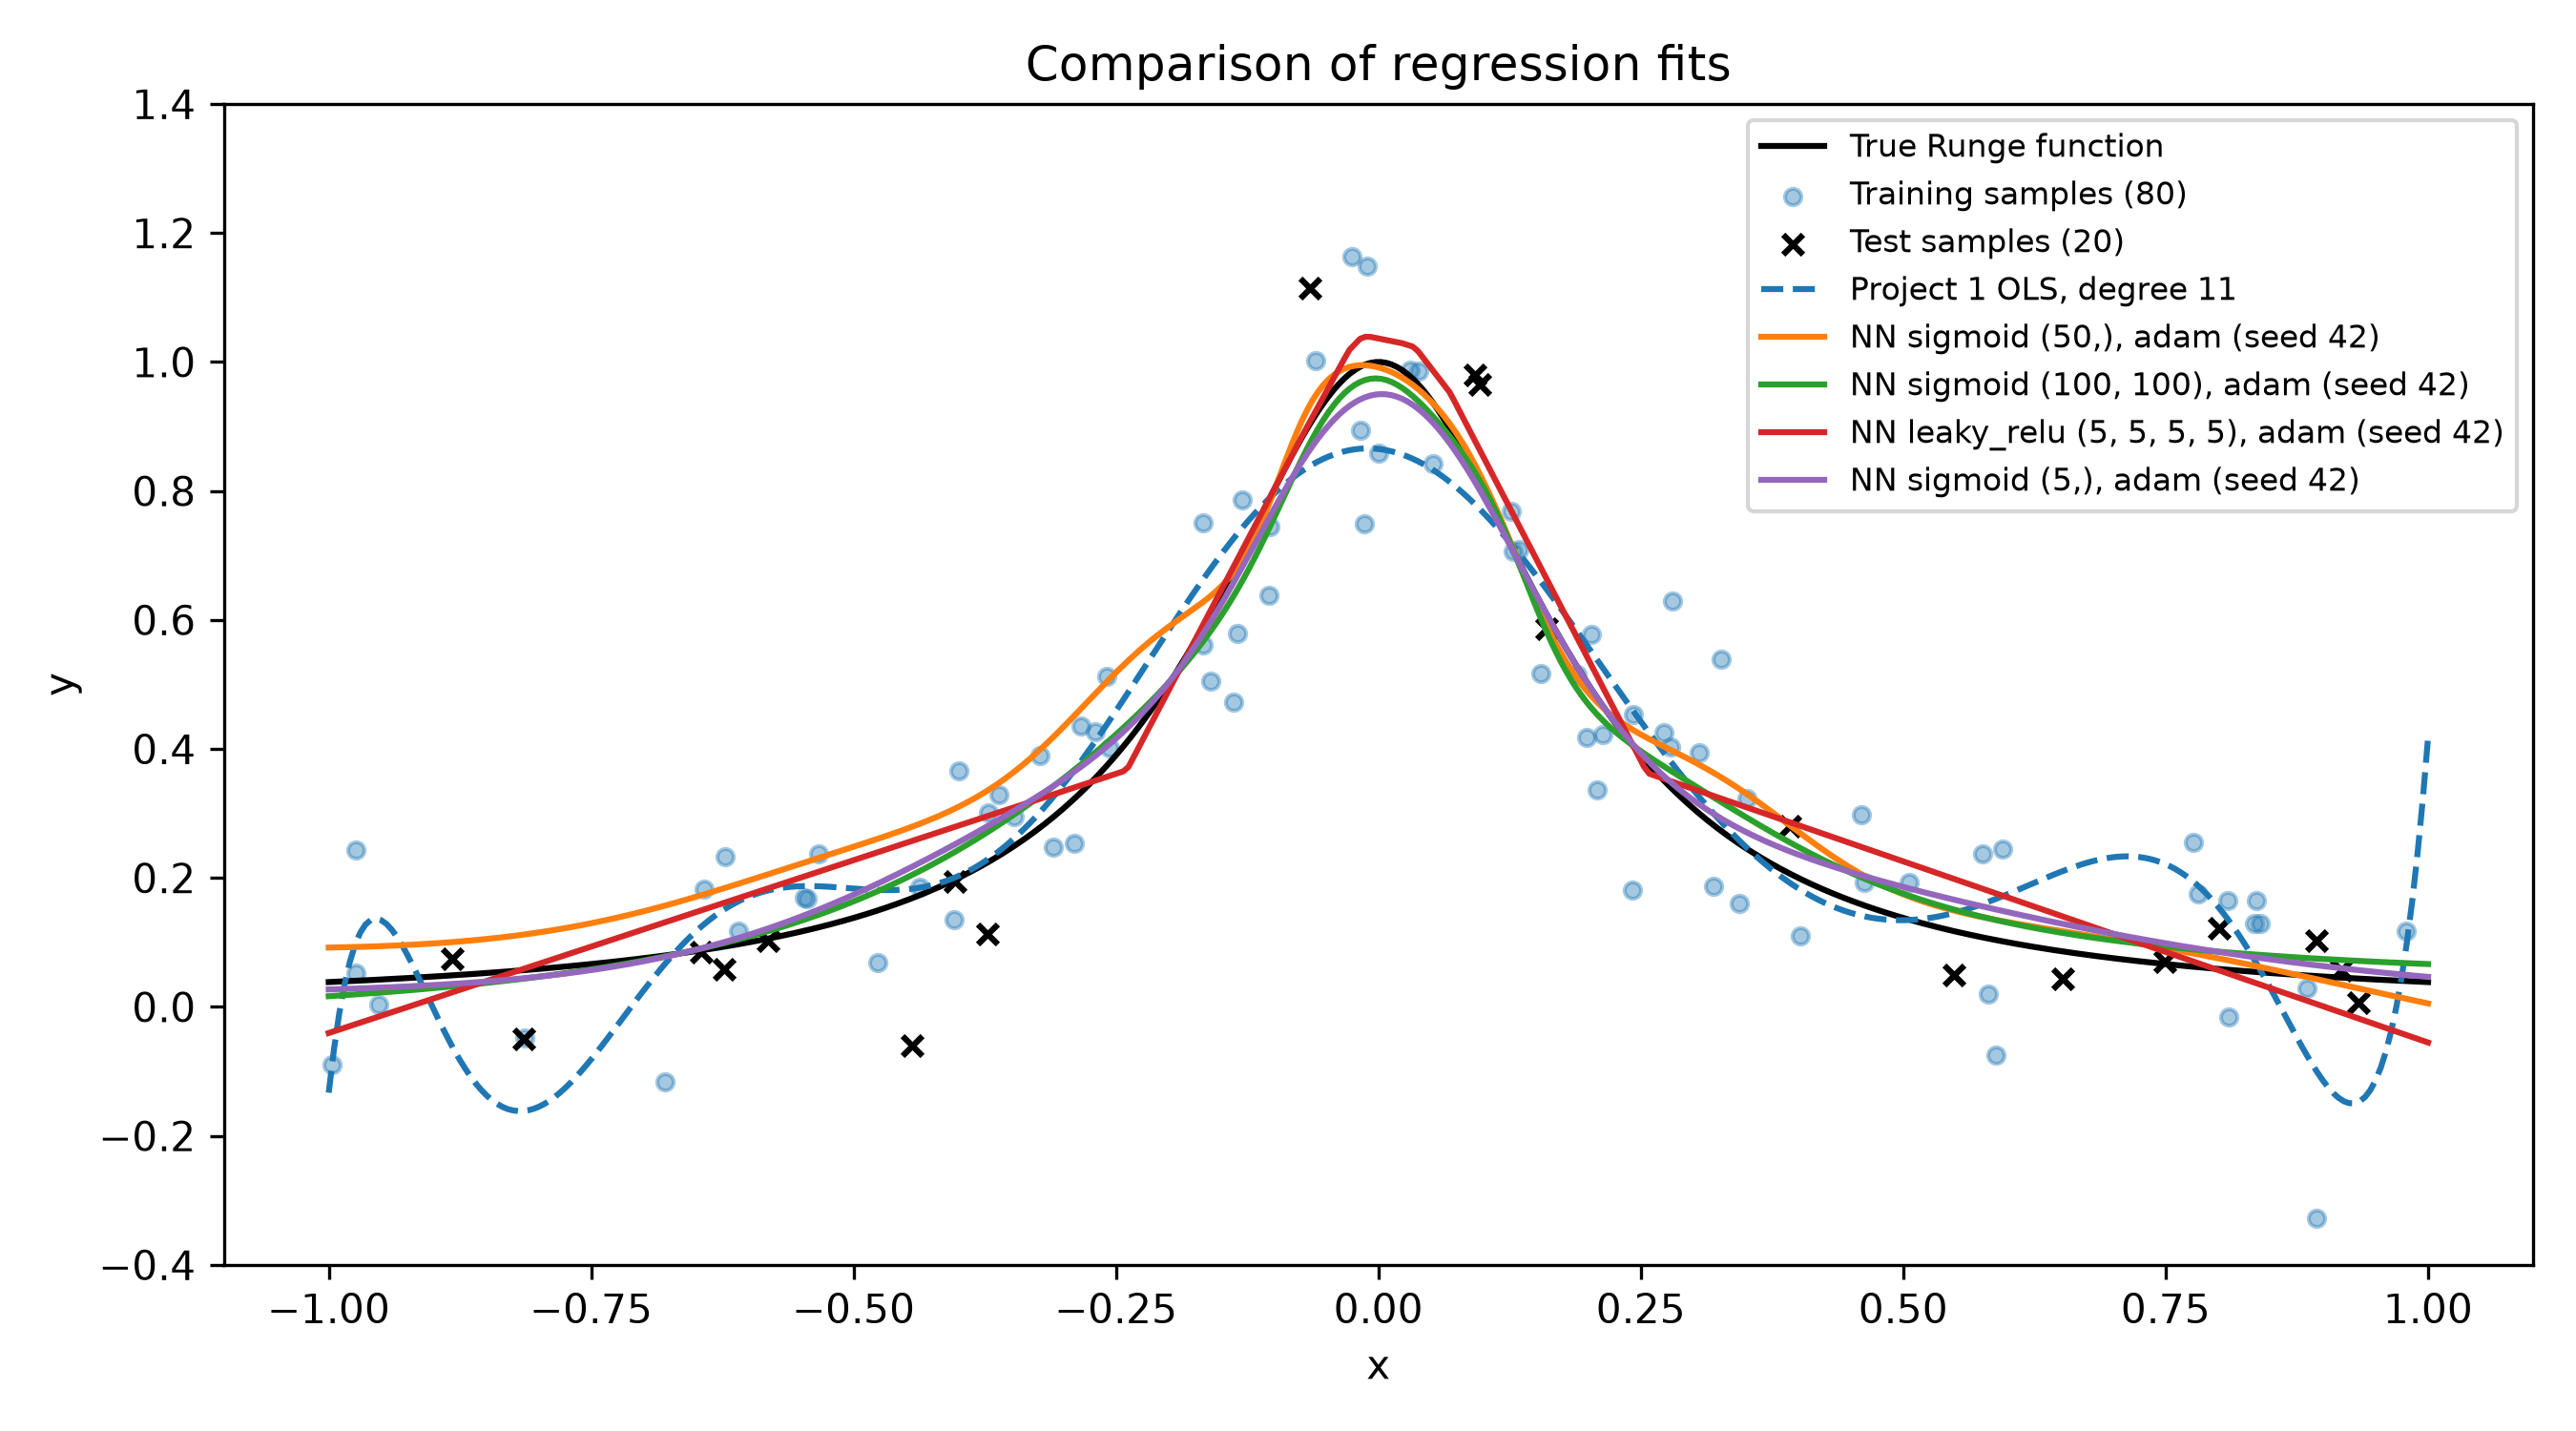
\includegraphics[width=\columnwidth]{figures/fig_part_c_fits.png}
\caption{Fits of OLS and four networks (seed 42) to the Runge function, with training and test points.}
\label{fig:fits}
\end{figure}

The networks with 16, 151, and 10\,401 parameters achieve test MSEs of $0.0127$–$0.0131$, compared with $0.0226$ for OLS. Their MSEs against the noise-free Runge function range from $0.0009$ to $0.0027$, substantially below the OLS error of $0.0088$. As shown in Figure~\ref{fig:fits}, the polynomial fit exhibits oscillations near the interval boundaries, which may contribute to its unusually high error in one CV fold. Ridge and Lasso reduce the CV MSE from $0.183$ to $0.0329$ and $0.0273$, respectively, and the test MSE to $0.0211$ and $0.0200$. Nevertheless, their test errors remain approximately $50$–$65\%$ higher than those of the three well-performing networks. 

The differences among these three networks are less conclusive. With only 20 test observations, the estimated sampling uncertainty of an MSE near $0.01$ is approximately $0.003$, exceeding the differences between their test errors. Evaluation against the noise-free function on 400 grid points provides an additional comparison without noise in the test targets. Although this measure favours the larger networks, the 16-parameter sigmoid network performs nearly as well as the 10,401-parameter network ($0.0010$ versus $0.0009$), while exhibiting the smallest standard deviation in test MSE across three random seeds ($0.0002$). This indicates that a considerably smaller network can achieve comparable accuracy on this regression task.

Notably, the network with the lowest CV MSE performs worst on the test set, achieving $0.0496\pm0.0570$ across three seeds and an MSE of $0.0269$ against the noise-free function. Its CV error is only about $0.0001$ below the second-best configuration, much smaller than the estimated standard error. This discrepancy illustrates the uncertainty associated with selecting the minimum from many CV estimates, where a small advantage in validation performance may not generalize. In contrast, the one-standard-error choice achieves substantially more stable test performance with only 16 parameters, highlighting the importance of accounting for uncertainty and model complexity during selection.

\subsection{$L_1$ and $L_2$ penalties}\label{sec:partd}

\begin{figure*}[t]
\centering
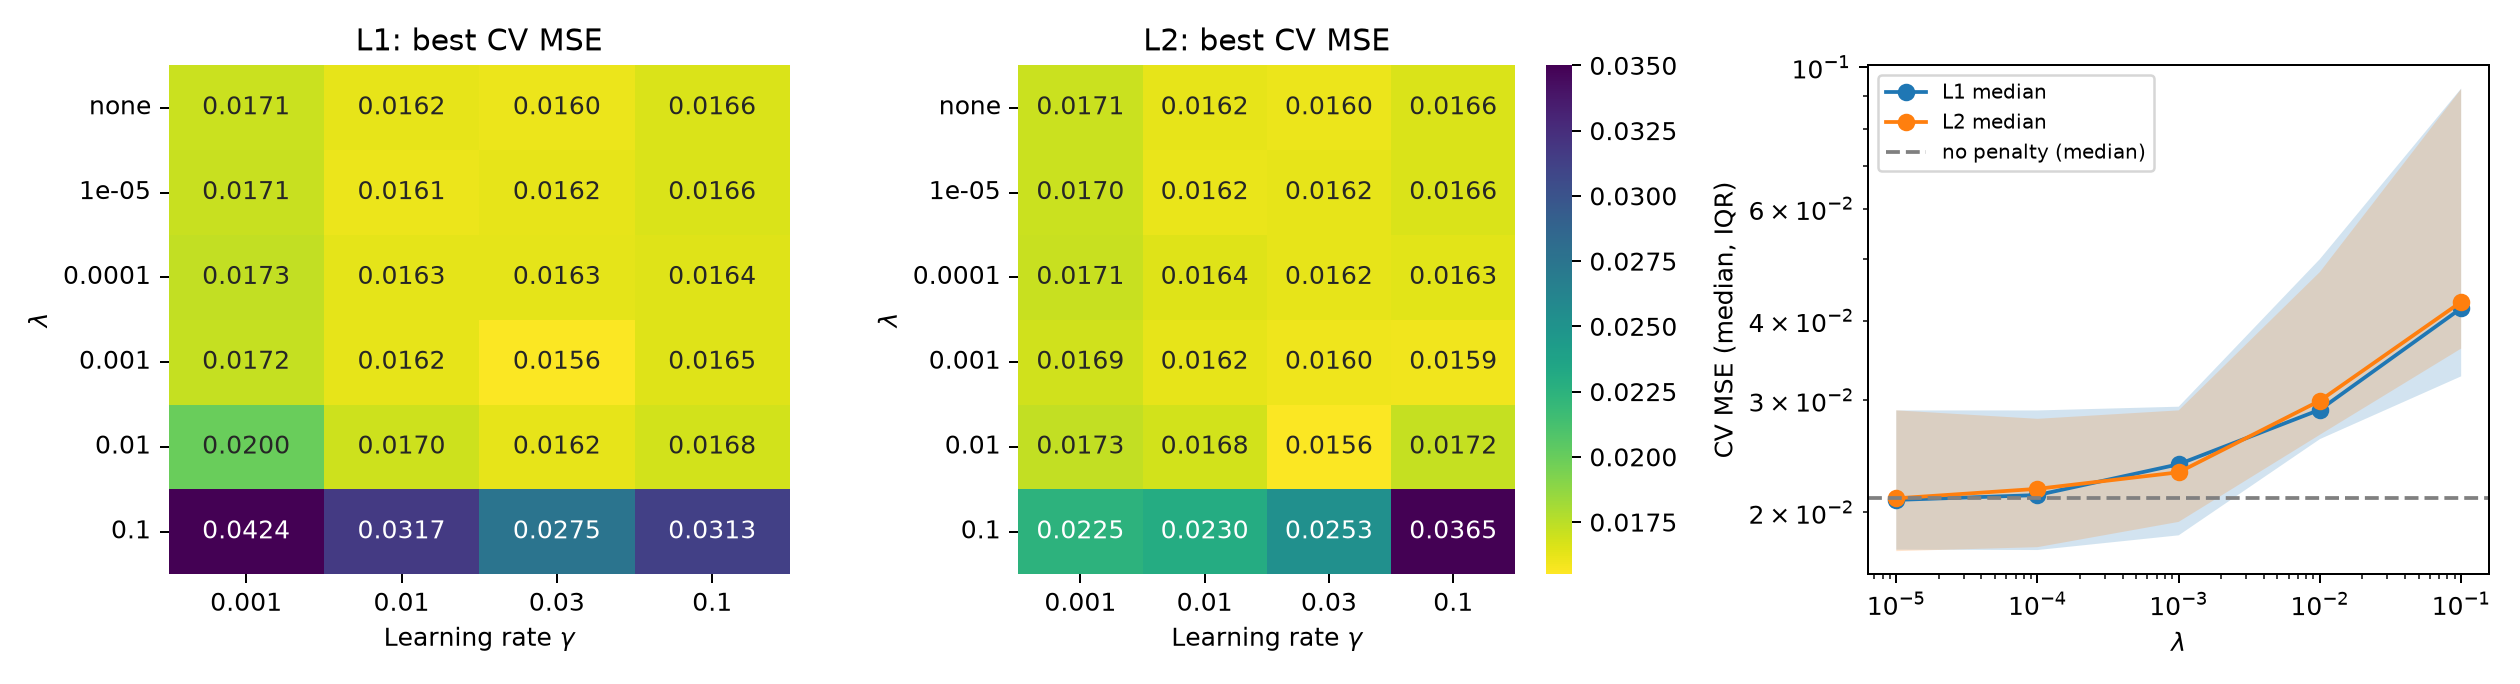
\includegraphics[width=\textwidth]{figures/fig_part_d_heatmap.png}
\caption{Left and middle: the lowest CV MSE over architecture, activation and optimizer for each pair of learning rate and $\lambda$ (the first row, ``none'', is the unpenalized case). Right: median and interquartile range of the CV MSE over all settings as a function of $\lambda$.}
\label{fig:dheat}
\end{figure*}


We investigate the effects of $L_1$ and $L_2$ regularization using the penalties defined in Eq.~\ref{eq:penalty}.  The experiment covers 1056 configurations, combining four network architectures ($(5,)$, $(10,)$, $(50,)$, and $(50,50)$), three activation functions, two optimizers (RMSprop and Adam), four learning rates ($10^{-3}$, $10^{-2}$, $3\times10^{-2}$, and $10^{-1}$), and five regularization strengths from $\lambda=10^{-5}$ to $10^{-1}$, alongside the unregularized case. Each configuration is trained for up to 250 epochs, with the results summarized in Figure~\ref{fig:dheat}.

The lowest CV MSEs are achieved with $L_1$ regularization at $\lambda=10^{-3}$ (leaky ReLU, $(50,50)$, Adam, $\gamma=0.03$) and $L_2$ regularization at $\lambda=10^{-2}$ (ReLU, $(50,50)$, RMSprop, $\gamma=0.03$), both reaching $0.0156$, compared with $0.0160$ for the best unregularized network. However, these differences are small relative to their standard errors of $0.003$–$0.004$. Of the 1056 configurations, 239 fall within one standard error of the best result, including 105 with $L_1$, 99 with $L_2$, and 35 without regularization. Figure~\ref{fig:dheat} also shows that penalties up to $\lambda=10^{-2}$ generally produce similar errors to the unregularized case, whereas stronger regularization at $\lambda=0.1$ increases the CV MSE to at least $0.0225$. The median CV error likewise increases with regularization strength, suggesting that excessive regularization leads to underfitting.

\begin{figure}[h]
\centering
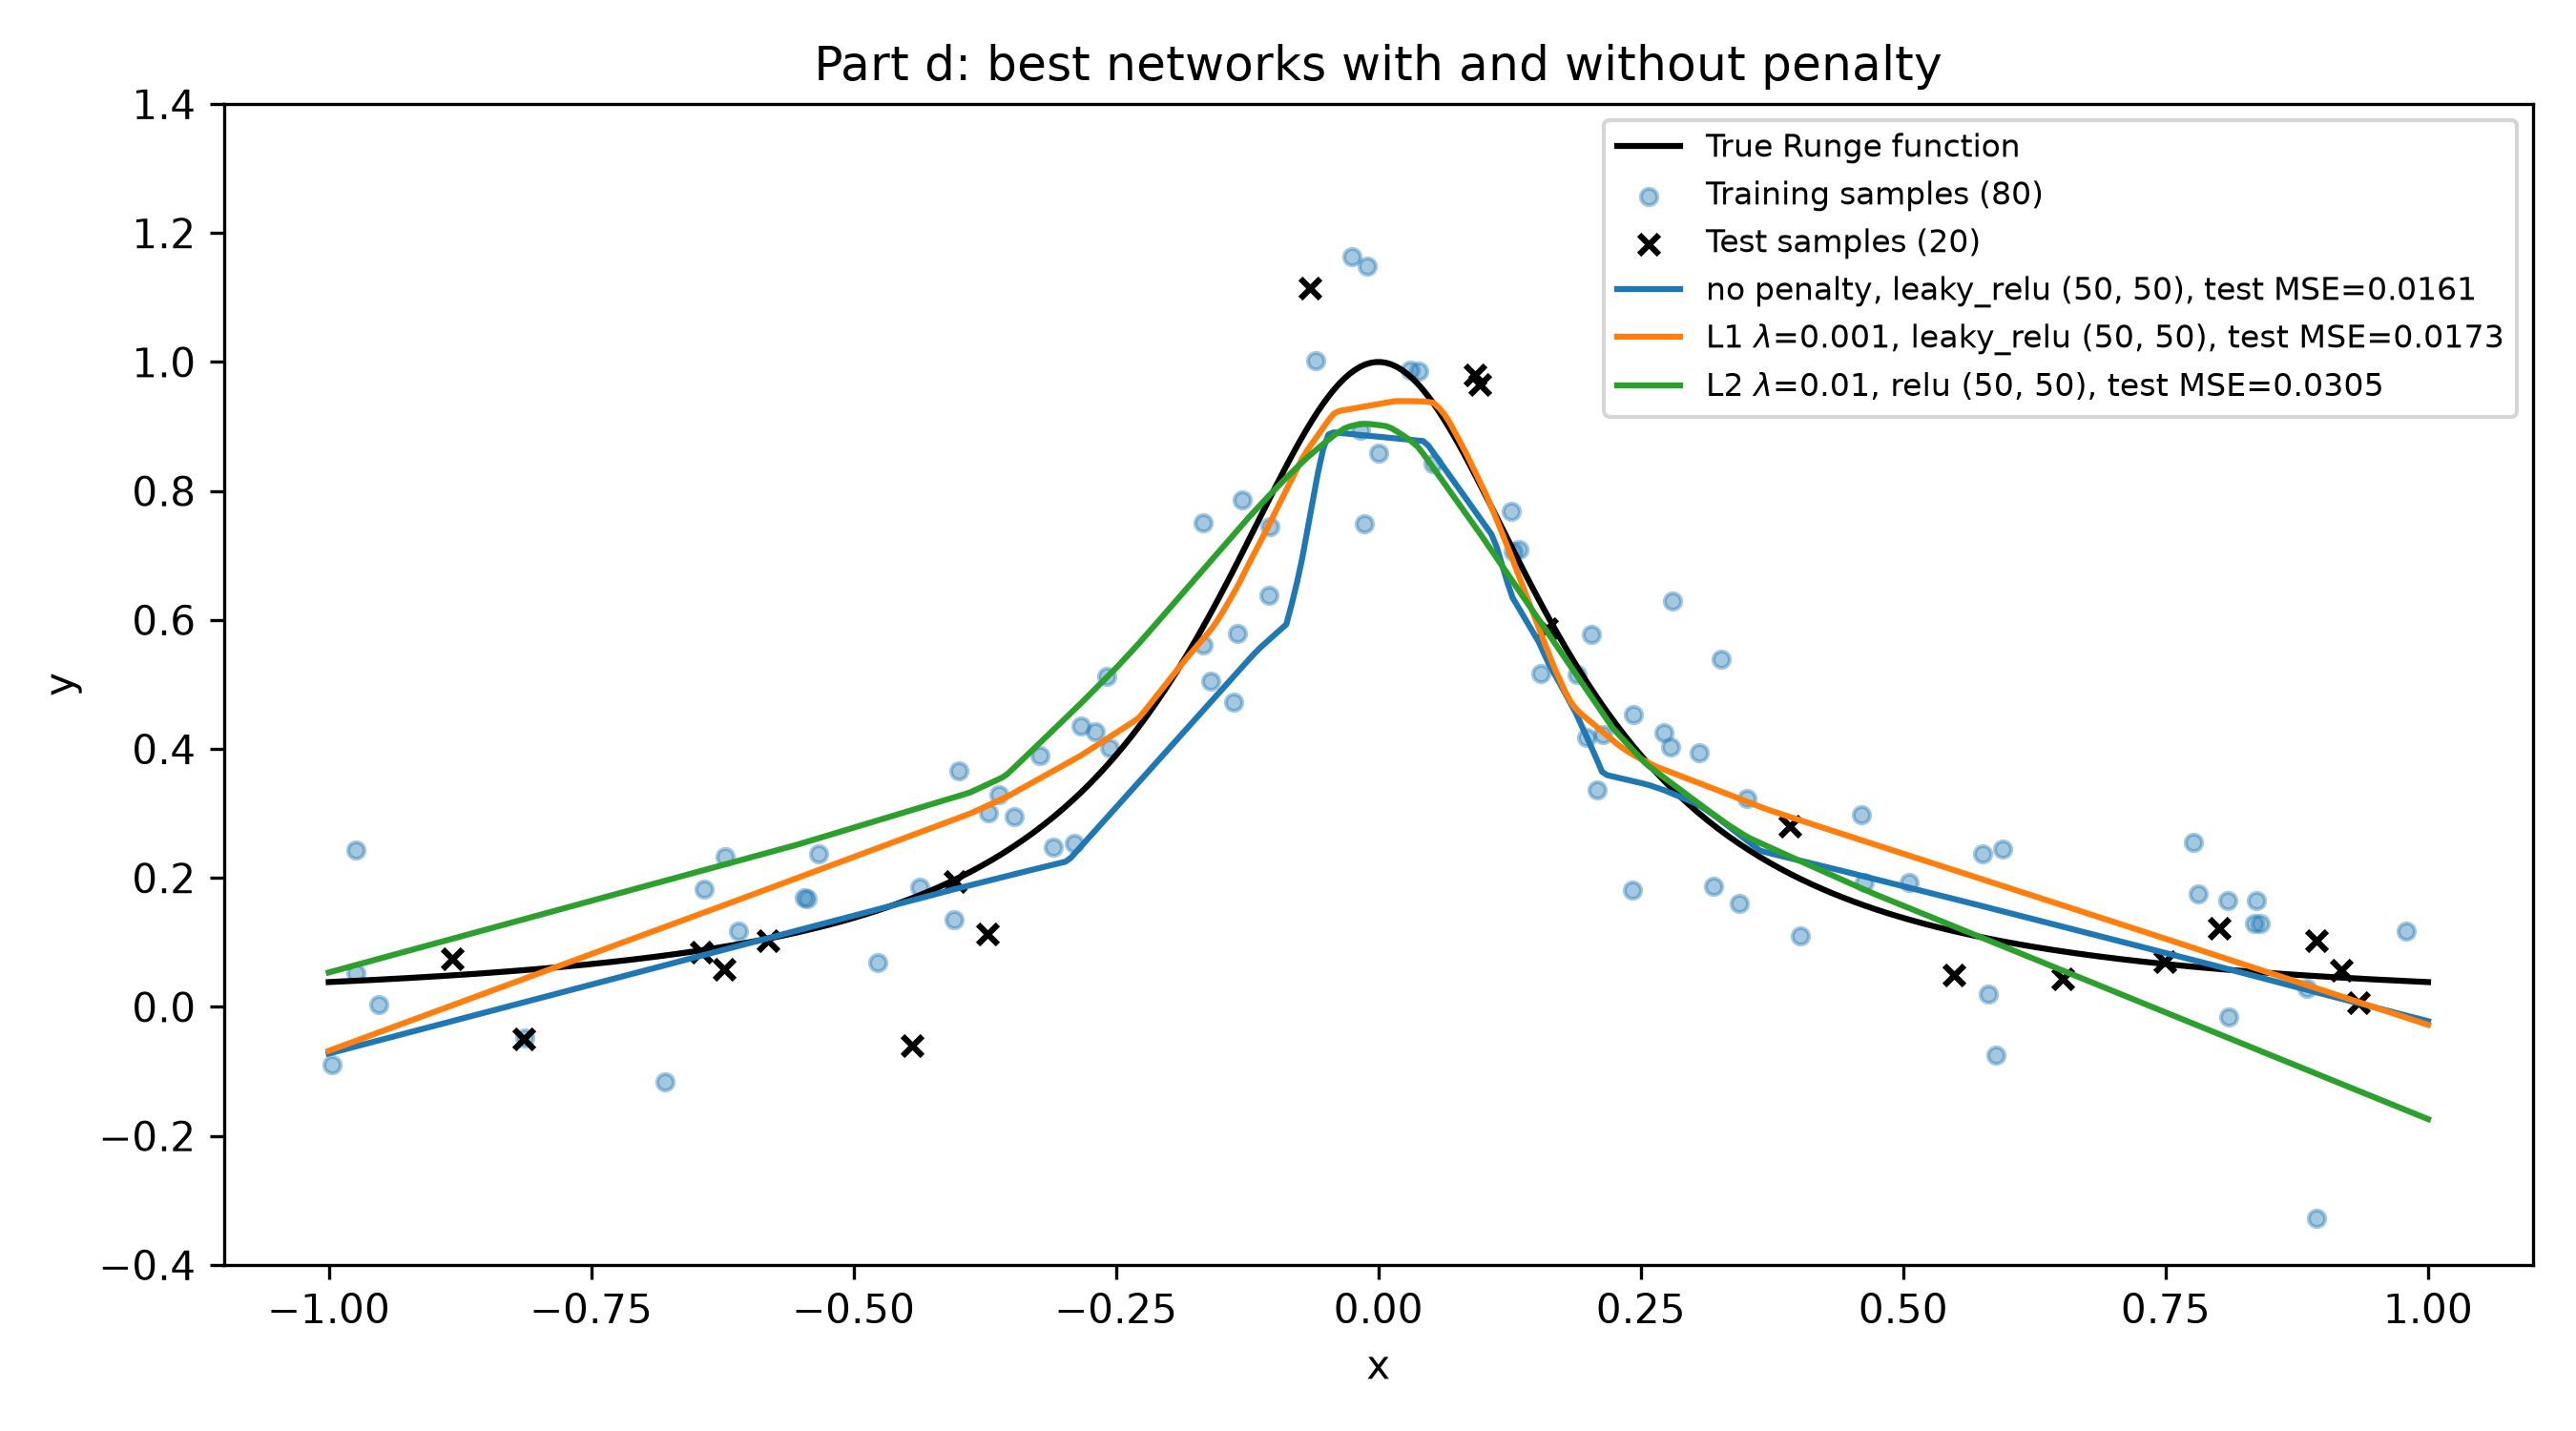
\includegraphics[width=\columnwidth]{figures/fig_part_d_fits.png}
\caption{Fits of the best unpenalized, $L_1$ and $L_2$ networks of the penalty scan (seed 42), evaluated on 400 grid points with the training and test points.}
\label{fig:dfits}
\end{figure}

Figure~\ref{fig:dfits} compares the fitted functions of the best unregularized, $L_1$-regularized, and $L_2$-regularized networks. Their test MSEs are $0.0161$, $0.0173$, and $0.0305$, respectively. All three underestimate the central peak of the Runge function, while the $L_2$ network also deviates noticeably near the right boundary, contributing to its higher test error. However, evaluating the predictions against the noise-free function on 400 grid points gives MSEs of $0.0047$, $0.0038$, and $0.0090$, respectively. Thus, although the unregularized network performs best on the noisy test set, the $L_1$ network provides a slightly closer approximation of the underlying function. This difference highlights the sensitivity of test-set comparisons to the limited number and distribution of observations, as discussed in Section~\ref{sec:comparison}.

Overall, the results provide no clear evidence that $L_1$ or $L_2$ regularization improves neural network performance under the tested conditions. Early stopping, examined in Section IV.C, may already limit overfitting, reducing the additional benefit of explicit penalties. Moreover, the regularized searches contain more configurations than the unregularized search, increasing the chance of obtaining a slightly lower minimum CV error. In contrast to the neural networks, Ridge and Lasso substantially improve upon unregularized polynomial regression, reducing the OLS CV MSE by factors of approximately $5.6$ and $6.7$, respectively. Figure~\ref{fig:summary} summarizes these differences in test performance, suggesting that the effectiveness of regularization depends on the model and training procedure.

\begin{figure}[h]
\centering
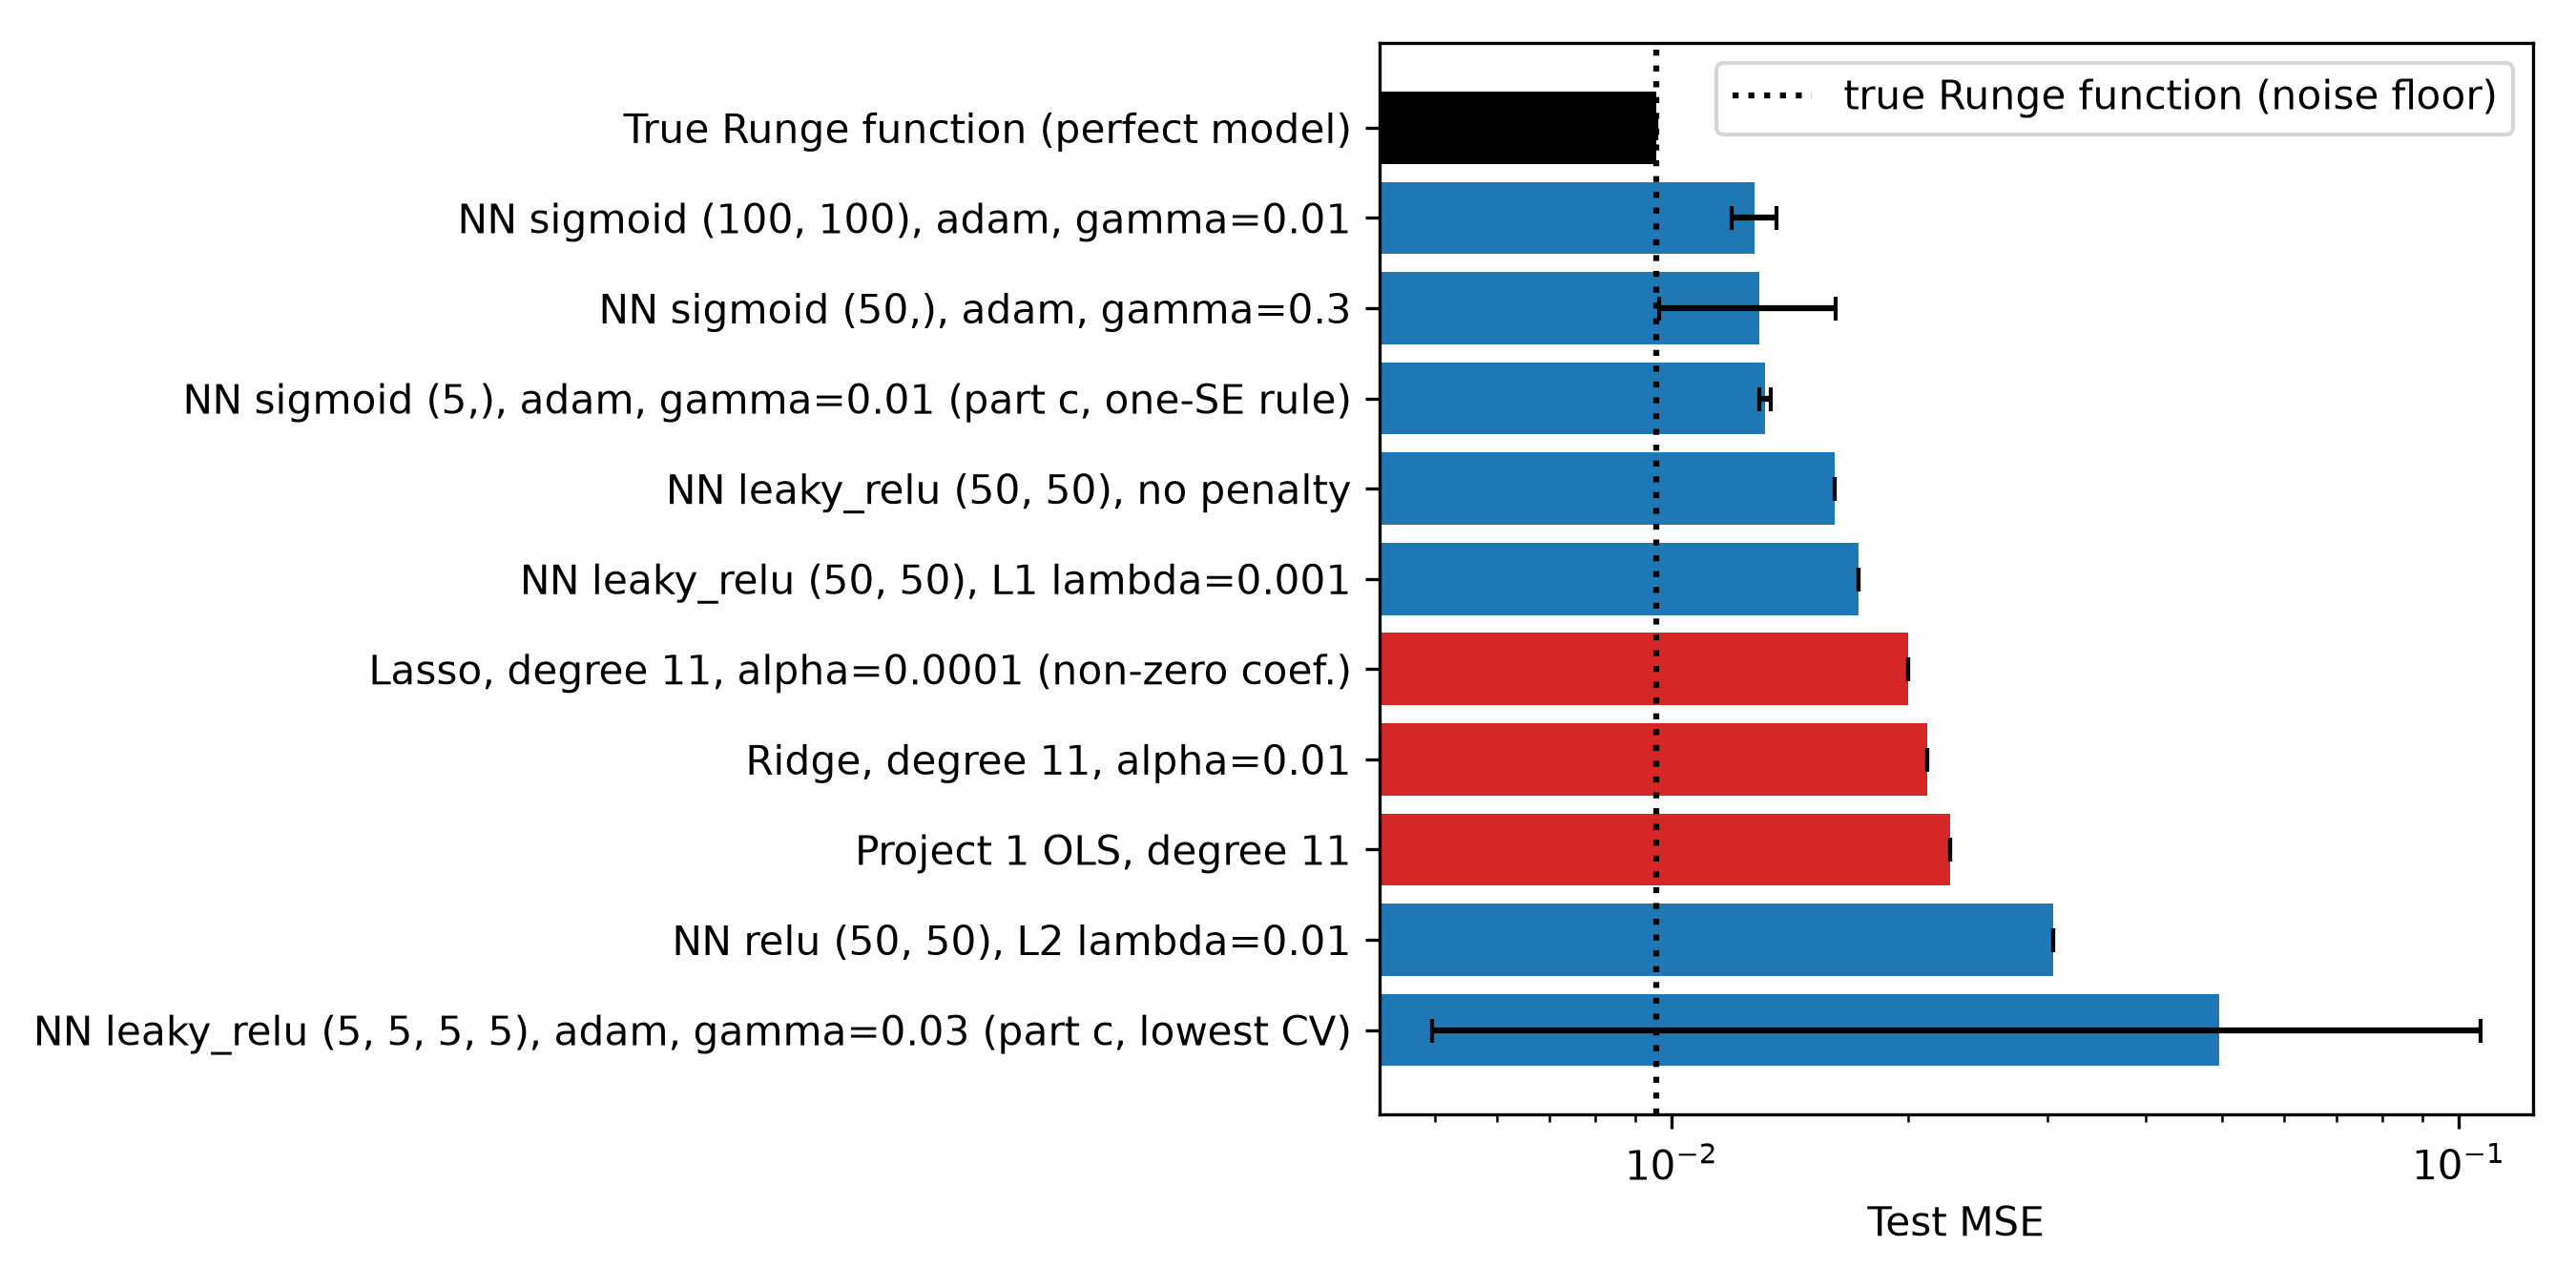
\includegraphics[width=\columnwidth]{figures/fig_summary_bar.png}
\caption{Test MSE of all regression models (logarithmic axis). Black: noise floor of the true function on the 20 test points; red: polynomial models of Project 1; blue: neural networks.}
\label{fig:summary}
\end{figure}

\subsection{Classification on MNIST}

\subsubsection{Logistic Regression Baselines}
Scikit-Learn's multinomial logistic regression achieves a test accuracy of $92.57\%$, while our network without hidden layers reaches $92.68\%$, both with 7,850 parameters. Their close agreement provides an end-to-end check of our softmax and cross-entropy implementation. Our model's validation accuracy stabilizes at $92.7$–$92.9\%$ after six epochs, consistent with the converged Scikit-Learn solver. This suggests that the remaining errors mainly reflect the limited capacity of a linear classifier rather than insufficient training.

\subsubsection{Initial Network Performance}
We first examine a network with one hidden layer of 128 ReLU nodes. Figure~\ref{fig:ecurves} shows that validation accuracy increases from $94.5\%$ after one epoch to $97.6$–$97.7\%$ after ten epochs, while training accuracy reaches $99.88\%$ at epoch 18. Although training loss continues to decrease to $0.010$, validation loss reaches its minimum of $0.080$ at epoch 13 before rising to $0.091$ at epoch 20. This indicates mild overfitting. The relatively stable validation accuracy suggests that continued training mainly affects prediction confidence rather than the predicted classes, since cross-entropy penalizes confident incorrect predictions more heavily.

\begin{figure}[h]
\centering
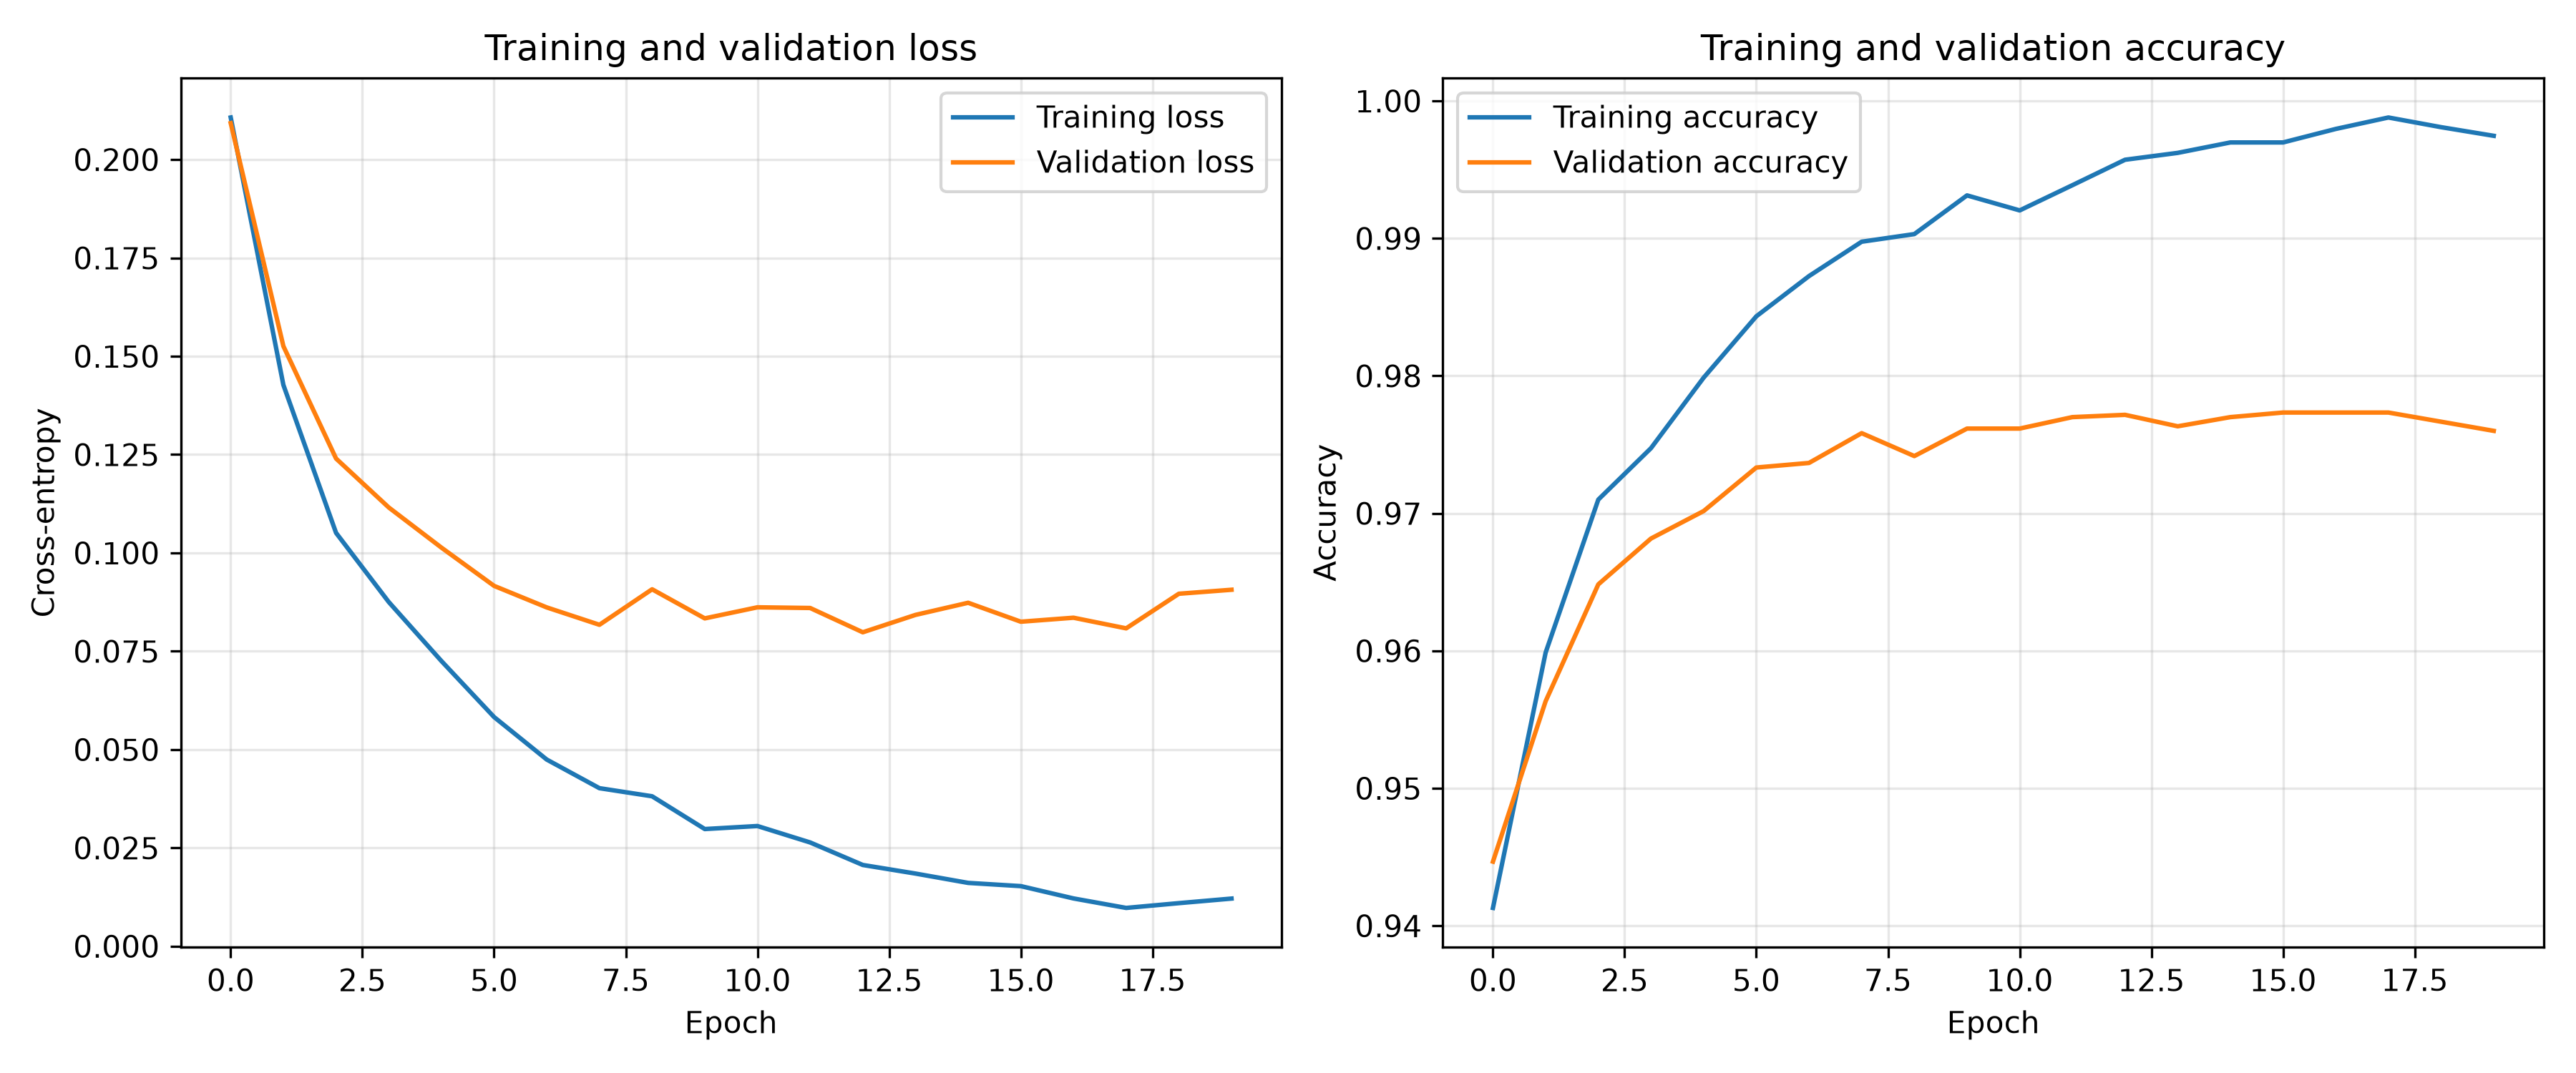
\includegraphics[width=\columnwidth]{figures/fig_part_e_curves.png}
\caption{Cross-entropy and accuracy on the training and validation sets for the network with one hidden layer of 128 ReLU nodes.}
\label{fig:ecurves}
\end{figure}

\subsubsection{Learning Rate and Regularization}
Figure~\ref{fig:val_acc} shows the effects of learning rate and $L_2$ regularization on the $(128,)$ ReLU network after ten epochs. The highest validation accuracy, $97.78\%$, occurs at $\gamma=3\times10^{-3}$ and $\lambda=10^{-5}$, compared with $97.62\%$ at the default $\gamma=10^{-3}$. As this difference is smaller than the estimated standard error of $0.2$ percentage points, we retain the default learning rate. Smaller rates, particularly $\gamma=3\times10^{-4}$, yield lower accuracies ($95.9$–$96.7\%$), suggesting slower convergence.

\begin{figure}[h]
\centering
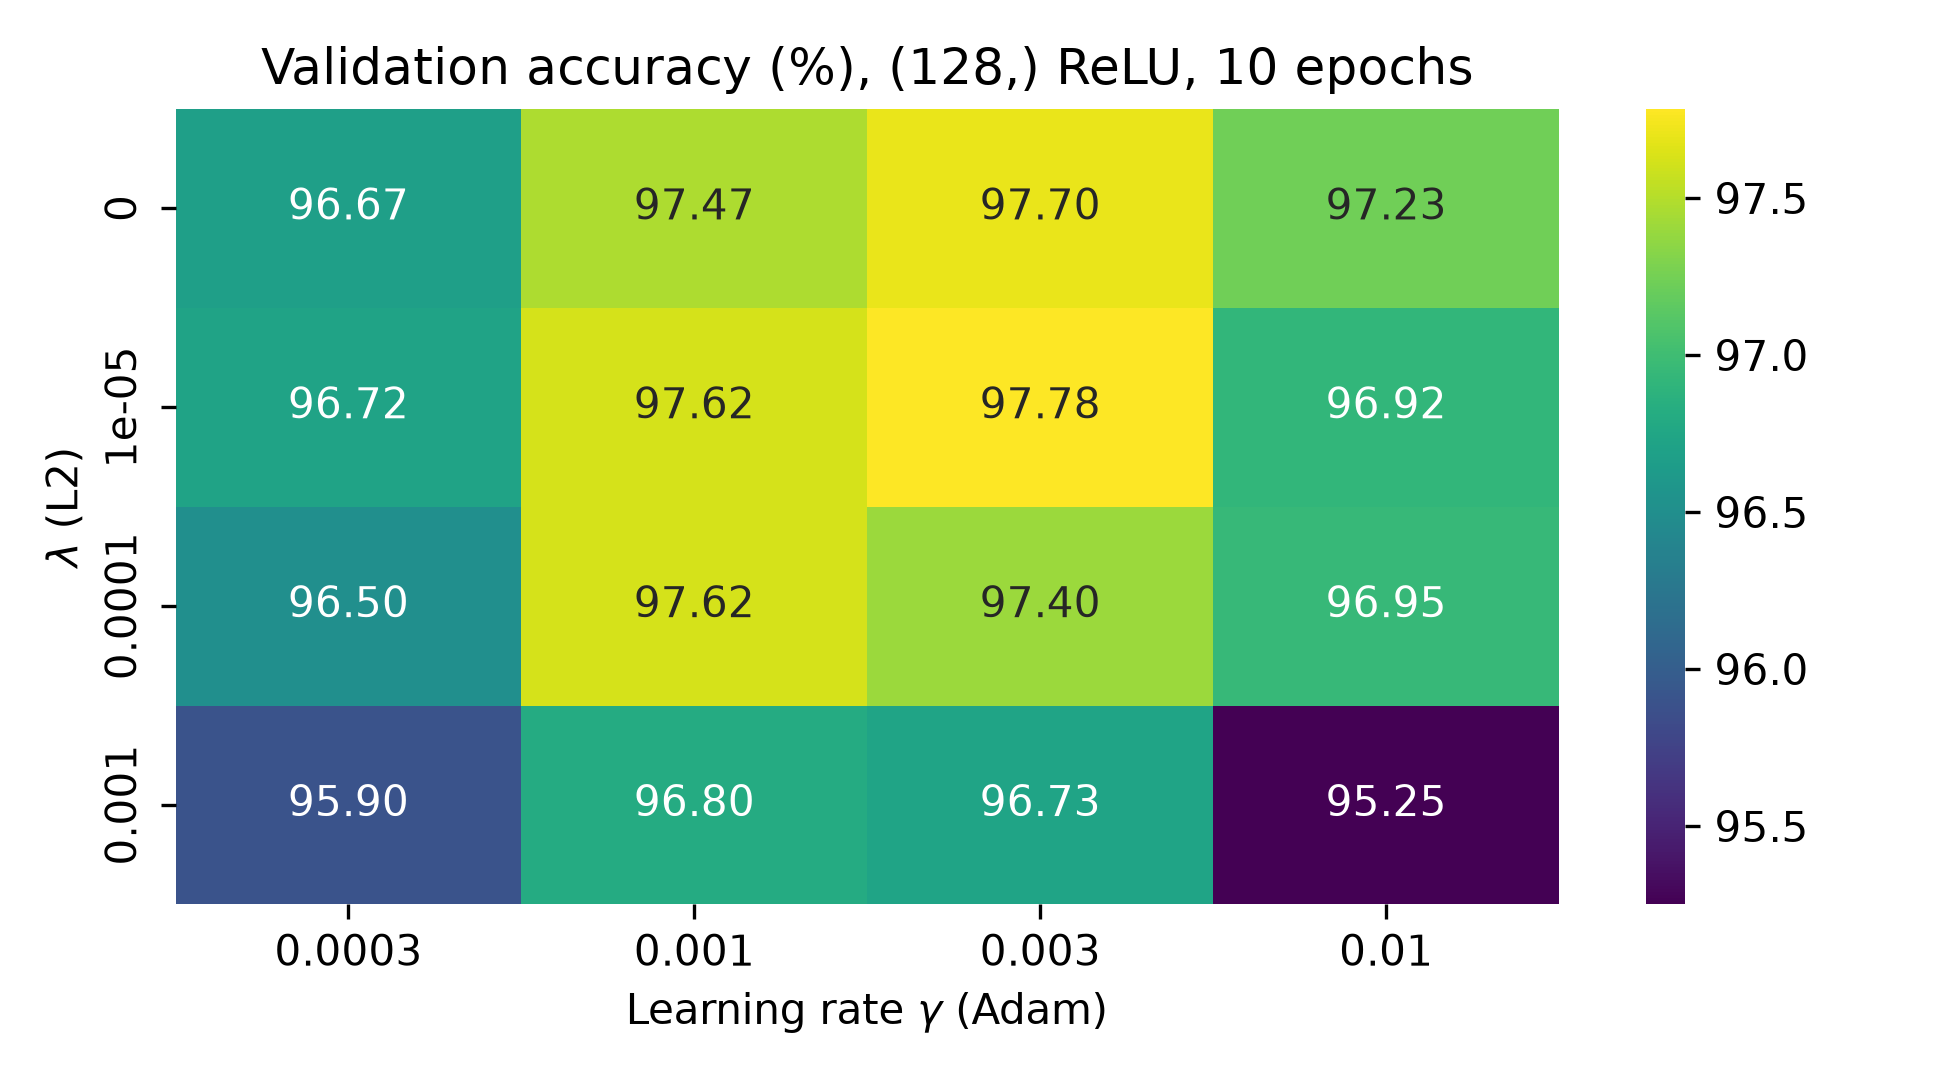
\includegraphics[width=\columnwidth]{figures/fig_part_e_gamma_lambda.png}
\caption{Validation accuracy (\%) of the network with one hidden layer of 128 ReLU nodes after 10 epochs, for each learning rate and $L_2$ strength (Adam, minibatches of 128).}
\label{fig:val_acc}
\end{figure}

For $\lambda\leq10^{-5}$, training accuracy reaches $99.3$–$99.7\%$, approximately two percentage points above validation accuracy. Increasing $\lambda$ to $10^{-3}$ narrows this gap but lowers both training ($95.3$–$97.2\%$) and validation ($95.3$–$96.8\%$) accuracy. Thus, stronger regularization provides no clear improvement under the tested conditions, although the fixed ten-epoch training period may also influence these results.

\subsubsection{Network Architectures and Activations}
Table~\ref{tab:e} compares five architectures after ten epochs. The three larger ReLU and leaky ReLU networks achieve similar validation accuracies of $97.62$–$97.75\%$, while the smaller $(64,)$ ReLU network reaches $97.17\%$. The $(128,)$ sigmoid network achieves $96.73\%$, approximately $0.9$ percentage points below its ReLU counterpart. However, since the learning rate was not tuned separately for sigmoid, this may reflect slower optimization rather than an inherent disadvantage of the activation function.

The small differences among the larger networks suggest limited gains from additional model capacity within the tested configurations. We select the $(128,64)$ ReLU network, with 109,386 parameters, based on its highest validation accuracy of $97.75\%$.

\begin{table}[h]
\centering
\begin{tabular}{llc}
\hline
\textbf{Hidden layers} & \textbf{Activation} & \textbf{Val.\ acc.} \\
\hline
(128, 64) & ReLU & $97.75\,\%$ \\
(128,) & leaky ReLU & $97.65\,\%$ \\
(128,) & ReLU & $97.62\,\%$ \\
(64,) & ReLU & $97.17\,\%$ \\
(128,) & sigmoid & $96.73\,\%$ \\
\hline
\end{tabular}
\caption{Validation accuracy of five networks (Adam, $\gamma=10^{-3}$, batch 128, $\lambda=10^{-5}$, 10 epochs).}
\label{tab:e}
\end{table}

\subsubsection{Test Performance and Model Comparison}
As shown in Table~\ref{tab:mnist_test}, the selected network achieves $97.56\%$ test accuracy (SE $0.15$ percentage points), compared with $92.57\%$ and $92.68\%$ for the logistic regression baselines. This reduces the classification error rate from approximately $7.4\%$ to $2.4\%$, a threefold reduction, although the network has nearly 14 times more parameters. Unlike the one-dimensional regression task, where a small network performs comparably to larger architectures, MNIST classification benefits substantially from nonlinear hidden layers. 

Our FFNN also achieves results comparable to Scikit-Learn's MLPClassifier, which reaches $97.73\%$ validation and $97.79\%$ test accuracy, compared with $97.75\%$ and $97.56\%$ for our implementation. This close agreement supports the reliability of our training procedure, although differences in weight initialization may contribute to the remaining gap. Moreover, Scikit-Learn's logistic regression was trained on all 60,000 images, compared with 54,000 for our FFNN, which should be considered when interpreting their performance.

\begin{table}[h]
\centering
\small
\setlength{\tabcolsep}{3pt}
\begin{tabular}{lrc}
\hline
\textbf{Model} & \textbf{Params} & \textbf{Test acc.} \\
\hline
Logistic regr., Scikit-Learn (\texttt{saga}) & 7850 & $92.57\pm0.26\,\%$ \\
Logistic regr., our code & 7850 & $92.68\pm0.26\,\%$ \\
Our network $(128,64)$ ReLU & 109\,386 & $97.56\pm0.15\,\%$ \\
Scikit-Learn MLP $(128,64)$ ReLU & 109\,386 & $97.79\pm0.15\,\%$ \\
\hline
\end{tabular}
\caption{Test accuracy on the 10\,000 MNIST test images, with the standard error $\sqrt{p(1-p)/n}$. Our models are trained on 54\,000 images, Scikit-Learn's logistic regression on all 60\,000.}
\label{tab:mnist_test}
\end{table}

\subsubsection{Classification Error Analysis}


The confusion matrix (Fig.~\ref{fig:confusion}) shows that the most frequent confusions are $4\to 9$ (21 images), $5\to 3$ (14), $7\to 2$ and $3\to 2$ (11 each) and $5\to 6$ (8). These errors mainly involve visually similar digits.

Digit 9 has the lowest precision ($95.8\%$), partly because other digits, particularly 4, are incorrectly classified as 9. In contrast, digits 5 and 4 have the lowest recall ($95.1\%$ and $96.2\%$, respectively), indicating that they are more frequently misclassified as other digits. Digit 1 achieves the highest F1 score ($0.992$), reflecting both high precision and recall. Overall, the five most frequent misclassification types account for 65 of the 244 test errors, showing that errors are not uniformly distributed across digit pairs. While these patterns suggest that visual similarity contributes to classification difficulty, the confusion matrix alone cannot determine whether the errors arise from ambiguous handwriting, insufficient training data, or limitations of the network architecture.

\begin{figure}[h]
\centering
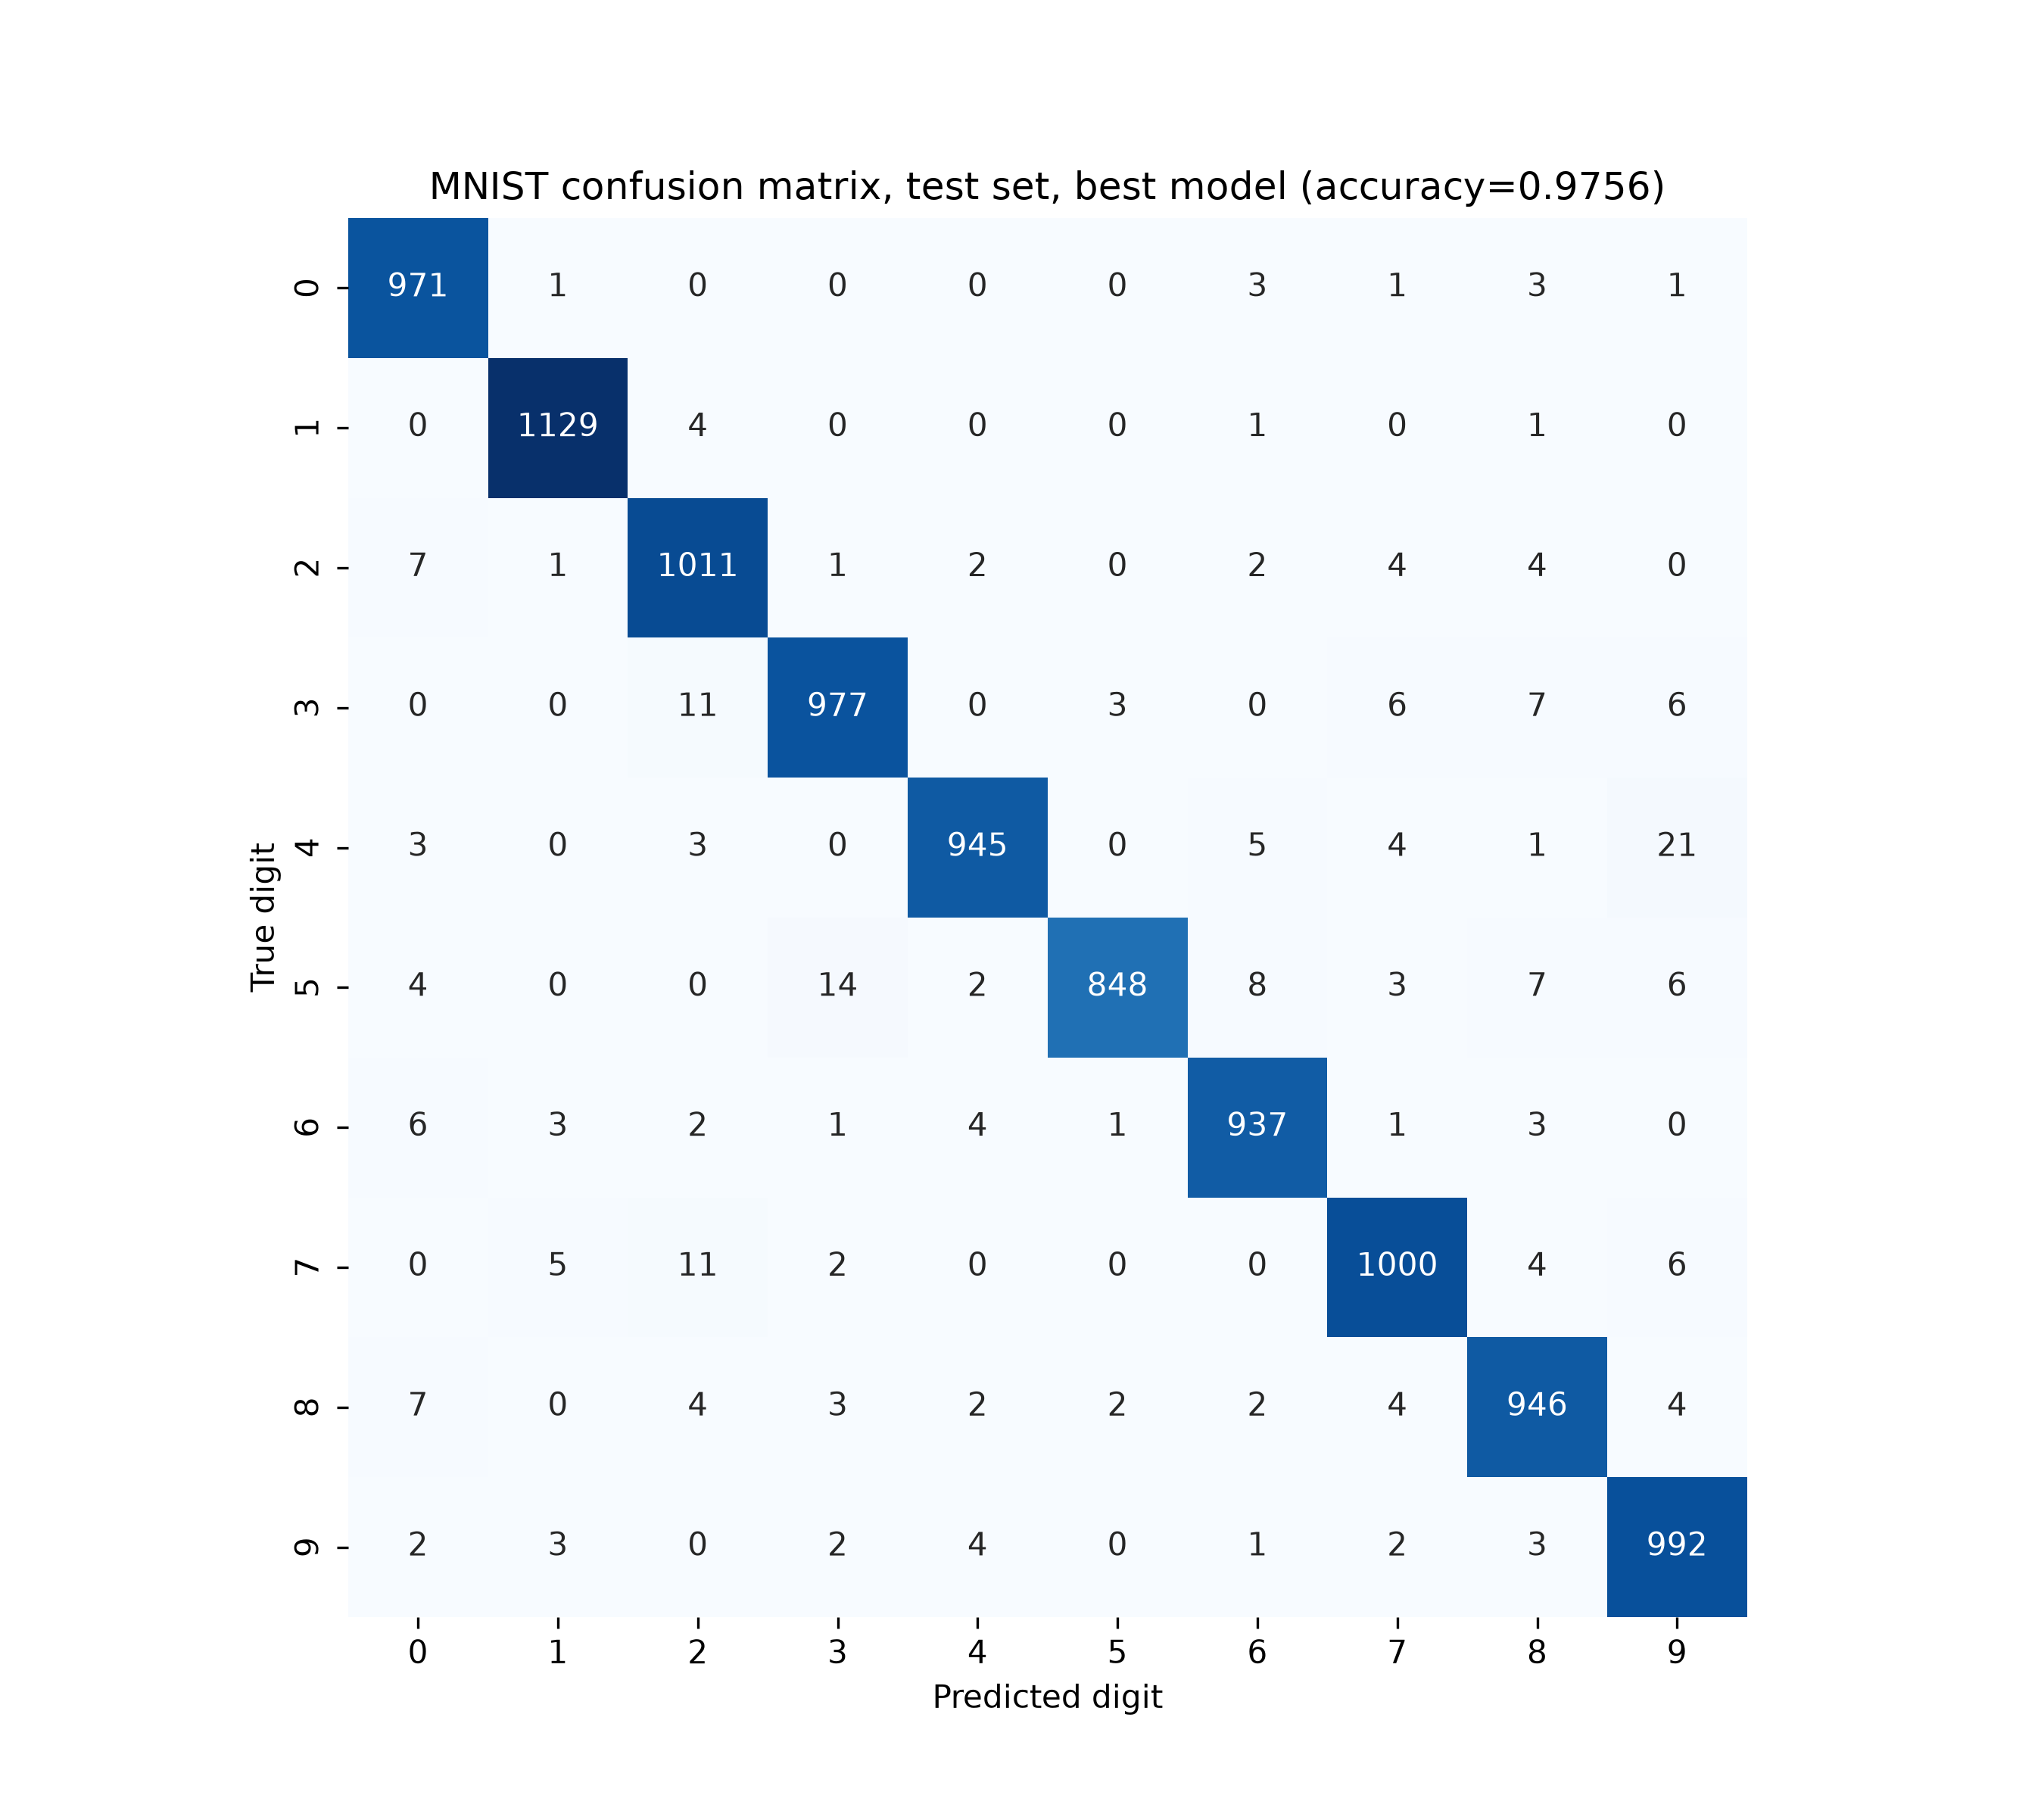
\includegraphics[width=\columnwidth]{figures/fig_part_e_confusion.png}
\caption{Confusion matrix of the selected network on the 10\,000 test images.}
\label{fig:confusion}
\end{figure}

\section{Discussion}\label{sec:discussion}
\subsection{Neural networks versus polynomial regression}
The regression results suggest that the advantage of neural networks is primarily due to their ability to learn nonlinear representations rather than simply having more parameters. As shown in Table~\ref{tab:final}, the 16-parameter sigmoid network achieves a test MSE of $0.0131$, compared with $0.0226$ for the 12-parameter OLS model, while the much larger 10,401-parameter network performs similarly ($0.0127$). This indicates that increasing model complexity does not necessarily improve generalization. Unlike polynomial regression, which uses a fixed basis of powers of $x$, neural networks learn their representations through hidden layers. The fitted curves in Figure~\ref{fig:fits} further suggest that learned representations help reduce the boundary oscillations observed in polynomial regression. However, these findings do not establish that neural networks are inherently better than polynomial regression, as the observed differences also depend on the choice of basis and regularization.

The improvement in predictive performance must also be considered alongside computational cost. OLS admits a closed-form solution, whereas neural networks require tuning of architectures, activations, optimizers, learning rates, and training duration. This is reflected in the 1,056 configurations evaluated in the regularization scan alone.  Furthermore, the Runge function is smooth, one-dimensional, and known, so alternative representations, such as splines, might achieve comparable accuracy with less tuning. The results therefore demonstrate an advantage over the polynomial models considered here, rather than establishing the general superiority of neural networks. Their benefits may be greater when suitable input features are difficult to define in advance, as in MNIST classification.

\subsection{Optimization and regularization}
The optimizer comparisons in Figure~\ref{fig:blr} and ~\ref{fig:bcurves}  indicate that optimization efficiency and predictive performance should be considered separately. Although the best configurations achieve similar CV errors ($0.0162$–$0.0182$), RMSprop and Adam reach their lowest validation errors after 167–840 epochs, while GD attains its lowest recorded error at the final epoch of 5000. The adaptive methods also perform well across wider ranges of learning rates, reducing the sensitivity of training to this hyperparameter. At excessively large learning rates, however, all methods can exhibit poor convergence or instability, with the effective range depending on network architecture. The adaptive updates may also help explain why wider sigmoid networks remain trainable despite the substantial gradient attenuation observed in Figure~\ref{fig:vanishing}, where the gradient norm decreases from approximately $2$ near the output to $10^{-7}$ in the first hidden layer. However, the effect of adaptive optimization on this behaviour was not isolated experimentally, so this explanation remains tentative.

The regularization results further show how its benefits depend on the model and training procedure. Ridge and Lasso reduce the OLS CV MSE from $0.183$ to $0.0329$ and $0.0273$, respectively, demonstrating the importance of controlling instability in polynomial regression. For neural networks, the best CV errors differ only slightly with and without explicit penalties ($0.0156$ versus $0.0160$), well within the estimated uncertainty. Figure~\ref{fig:overfit} provides a possible explanation, as the increasing validation error during prolonged training indicates that early stopping can help limit overfitting before explicit penalties become necessary. This effect was not isolated in a controlled comparison, so the contribution of early stopping to the limited benefit of $L_1$ and $L_2$ regularization remains uncertain. The MNIST experiments show a similar limitation of stronger regularization, where narrowing the training–validation gap also reduces both accuracies.

\subsection{Model selection and generalization}
The architecture scan indicates that greater complexity does not necessarily improve predictive performance. As shown in Figure~\ref{fig:depthwidth}, 66 of 75 configurations fall within one standard error of the best CV result. The poorer results are concentrated among narrow ReLU and deep narrow sigmoid networks, consistent with dead ReLU units and vanishing gradients, respectively. Although dead units were not measured directly, these patterns suggest that optimization difficulties can limit performance even when a network has sufficient capacity.

The model-selection results also show that a lower CV-error does not always mean better test performance. The leaky ReLU network with the lowest CV MSE ($0.0159$) achieves a test MSE of $0.0496\pm0.0570$ across three seeds. By comparison, the one-standard-error rule selects a simpler 16-parameter network with a lower and more consistent test MSE ($0.0131\pm0.0002$). This difference suggests that small improvements in CV error may be unreliable when selecting among many settings, supporting the use of simpler models when their validation performance is comparable.

With only 20 test points, small differences in regression performance are difficult to assess reliably. The three well-performing networks differ in test MSE by less than $0.0005$, much smaller than the approximate sampling uncertainty of $0.003$. Figure~\ref{fig:dfits} illustrates this uncertainty: the $L_1$-regularized network has a slightly higher test MSE than the unregularized network ($0.0173$ versus $0.0161$), but approximates the noise-free Runge function more accurately ($0.0038$ versus $0.0047$). Thus, model rankings based on a small, noisy test set may not accurately reflect how well each model approximates the true function.


\subsection{Classification}
The MNIST results demonstrate a clearer benefit from nonlinear hidden representations than the one-dimensional regression task. The selected FFNN achieves $97.56\%$ test accuracy, compared with $92.57\%$ for logistic regression, reducing the classification error rate from approximately $7.4\%$ to $2.4\%$. Although the FFNN requires nearly 14 times more parameters, the additional capacity appears useful for capturing nonlinear relationships among image pixels. Its close agreement with Scikit-Learn's MLPClassifier ($97.79\%$) further supports the reliability of our implementation, although differences in initialization and training procedures prevent a strictly equivalent comparison.

The confusion patterns in Figure~\ref{fig:confusion} suggest that visually similar digits remain difficult to distinguish, particularly digits 4 and 9. Since the network operates on flattened images, it does not explicitly exploit spatial relationships between neighbouring pixels. Convolutional neural networks could potentially improve classification by incorporating local connectivity and weight sharing, although this was not investigated.

\subsection{Limitations}
The main limitation of the regression experiments is the small dataset, particularly the 20-point test set, which makes model comparisons sensitive to sampling variability. Although the main regression networks were evaluated across three initializations, the final regularization models used only one, making it difficult to distinguish the effects of penalties from initialization. Furthermore, selecting the lowest validation error across epochs and numerous hyperparameter configurations may introduce optimism into the CV estimates.

For MNIST, learning rates and regularization strengths were tuned on a single architecture before comparing five configurations under a fixed training budget. Consequently, differences between architectures and activation functions may partly reflect their sensitivity to the chosen hyperparameters rather than their full predictive potential. The experiments therefore provide a comparison of the tested configurations, rather than an exhaustive assessment of the best achievable performance.

\section{Conclusion}\label{sec:conclusion}
We implemented a feed-forward neural network (FFNN) from scratch and verified its gradients against JAX automatic differentiation and finite differences. Across regression and classification tasks, the networks demonstrated the benefits of learned nonlinear representations. On the Runge function, they outperformed the polynomial models from our previous project, achieving a test MSE of approximately $0.013$ compared with $0.020$–$0.023$ for the polynomial baselines. On MNIST, the selected network achieved $97.56\%$ test accuracy, compared with $92.57\%$ for logistic regression.

The regression experiments showed that relatively small networks could perform as well as much larger ones, making additional complexity unnecessary for this problem. RMSprop and Adam converged more efficiently than gradient descent, while early stopping reduced overfitting during prolonged training. Unlike Ridge and Lasso in polynomial regression, $L_1$ and $L_2$ penalties provided no clear additional improvement for the neural networks under the tested conditions. The poor test performance of the lowest-CV configuration also highlighted the importance of accounting for validation uncertainty when selecting models. Overall, these findings suggest that network performance depends on both the suitability of the learned representation and the reliability of the training and selection procedures.

\subsection*{Future work}
Future work could compare neural networks with alternative regression bases, such as splines, and investigate the stability of model selection using additional random initializations and test data. For MNIST, further architecture-specific tuning and convolutional neural networks could be explored to assess the benefits of incorporating spatial information.


\appendix
%TC:ignore
\section{Use of LLM Tools}
\subsection{Tools used}
The following large language model tools were used during the
development of this report:
\begin{itemize}
    \item \textbf{Claude} (\url{claude.ai}, October 2026)
    \item \textbf{ChatGPT} (\url{chatgpt.com}, October 2026)
\end{itemize}

\subsection{LLM declaration}
Table~\ref{tab:llm-text} reports the level of LLM assistance for each
section of the report.
Table~\ref{tab:llm-code} reports the level of LLM assistance for each
code file or notebook. All code belongs to the \texttt{Project2.ipynb} notebook and to the files \texttt{scratch\_ffnn.py} and \texttt{scratch\_classifier.py}.

\begin{table*}[t]
    \centering
    \small
    \begin{tabular}{p{0.16\textwidth}p{0.06\textwidth}p{0.7\textwidth}}
        \hline
        \textbf{Section} & \textbf{Level} & \textbf{Notes} \\
        \hline
        Abstract
        & 1
        & ChatGPT was used for minor phrasing and polishing. \\

        \hline
        Introduction
        & 1
        & ChatGPT was used for minor phrasing and polishing. \\

        \hline
        Methods
        & 1
        & ChatGPT was used for minor phrasing and polishing. \\
        
        \hline
        Implementations
        & 1
        & ChatGPT was used for minor phrasing and polishing. \\
        
        \hline
        Results
        & 1
        & ChatGPT was used for minor phrasing and polishing. \\

        \hline
        Conclusion
        & 2
        & ChatGPT was used to better structure the sentences. Content was provided by us. \\ 
        \hline
     \end{tabular}
    \caption{LLM assistance in text writing and editing.}
    \label{tab:llm-text}
\end{table*}

\begin{table*}[t]
    \centering
    \small
    \begin{tabular}{p{0.16\textwidth}p{0.06\textwidth}p{0.7\textwidth}}
        \hline
        \textbf{Part} & \textbf{Level} & \textbf{Description} \\
        \hline
        Part a) & 0 & Analytical part; no code. \\
        \hline
        Part b) & 2 & Claude spotted that the gradient-check \texttt{assert} ignored the finite-difference result, which we fixed. Claude suggested printing the per-fold OLS errors. \\
        \hline
        Part c) & 1 &  Claude suggested the vanishing-gradient and overfitting analyses and pointed out that the learning rate should be tuned per activation \\
        \hline
        Part d) & 2 & Claude identified four bugs (diverged folds hidden in the CV average, Ridge/Lasso $\alpha$ chosen on the test set, epochs not rescaled in the final training, handling of \texttt{penalty="none"}) and supplied the fixes, the Lasso convergence check and the corrected plotting code for Fig.~10, which we integrated and verified. \\
        \hline
        Part e) & 2 & Claude identified three bugs (labels of the full training set used with the reduced feature matrix, scaling cell not idempotent, test set used before model selection) and helped with the fixes \\
        \hline
        Part f) & 2 & Claude supplied the extension of the summary table with the error against the noise-free function. \\
        \hline
        \texttt{scratch\_\allowbreak ffnn.py} & 1 & Claude suggested checking the gradients against finite differences and storing the training history for cross-validation. \\
        \hline
        \texttt{scratch\_\allowbreak classifier.py} & 2 & Claude supplied the $L_1$ option and \texttt{check\_gradients}, which we integrated and tested. \\
        \hline
    \end{tabular}
    \caption{LLM assistance in code generation and development.}
    \label{tab:llm-code}
\end{table*}
%TC:endignore

\bibliographystyle{apsrev4-1}
\bibliography{bibliography}  
\end{document}
